% ADD ./styles DIRECTORY TO TEXINPUTS AND BSTINPUTS!!!!

\documentclass[a4paper,12pt,oneside]{book}
\usepackage[american]{babel}			% American hyphenation
\usepackage[latin1]{inputenc}			% Recognizes special characters (accented letters, etc.)
\usepackage[pdftex]{graphicx}			% Allows the use of images through \includegraphics
\DeclareGraphicsExtensions{.pdf, .png, .jpg, .gif, .bmp}
\usepackage{verbatim}				% Allows the use of the comment environment
\usepackage{paralist}				% Allows the use of inparaenum
\usepackage{algorithm2e}			% Allows the use of the algorithm environment
\usepackage[amssymb]{SIunits}			% Allows to use the symbols for SI units
\usepackage{numprint}				% Allows to use advanced formatting for numbers
\usepackage{amsthm}				% Allows the use of the defn environment
\usepackage{amsmath}				% Introduces advanced mathematical notations
\usepackage{amssymb}				% Introduces various math symbols
%\usepackage{wasysym}				% Introduces the WASY symbols
\usepackage{bibentry}				% BibTeX

\usepackage{fancyhdr}				% Introduces the Fancy style
\usepackage[pdftex,plainpages=false,pdfpagelabels,colorlinks,linkcolor=black,citecolor=black,filecolor=black,urlcolor=black]{hyperref}
% Introduces the hypertextual references on the document. THIS SHOULD BE THE LAST INSERTED PACKAGE!

\setlength{\headheight}{15pt}			% Sets the height of the header
\setlength{\parindent}{5mm}			% Sets the indentation of new paragraphs
\linespread{1.2}				% Sets the line height
\makeindex					% Starts the collection of the words between \index{} to create the Index

\begin{document}

\hypersetup{pdfauthor={Fabio Arlati, Antonio Miele},pdftitle={ReSP User Manual}}
\hypersetup{bookmarksopen}			% Sets author, title, and options in the PDF properties
\pagestyle{empty}				% Sets the style 'empty' for the title page

\begingroup
  \renewcommand{\thepage}{title}		% Used to have a single #1 page (hyperref rises a warning)
  \title{\Huge \textit{\textsc{ReSP User Manual}\thanks{Special thanks to Giovanni Beltrame and Luca Fossati for developing the core of this tool}}}
  \author{	Fabio Arlati - \href{mailto:arlati.fabio@gmail.com}{arlati.fabio@gmail.com} \and
		Antonio Miele - \href{mailto:miele@elet.polimi.it}{miele@elet.polimi.it} \and
		Francesco Bruschi - \href{mailto:bruschi@elet.polimi.it}{bruschi@elet.polimi.it} }
  \date{June 2010}
  \maketitle					% This and the commands above are used to make the original LaTeX title
\endgroup

\frontmatter					% Used only by book documents
\pagenumbering{Roman}				% Uppercase letters for page numbers
\pagestyle{plain}				% Sets the style 'plain' for the indexes

\tableofcontents
%\listoffigures

\mainmatter					% Used only by book documents
\pagenumbering{arabic}				% Numeric page numbers
\fancyhead{}
\fancyfoot{}
\fancyhead[OR]{\slshape \leftmark}
\fancyhead[OL]{}
\fancyfoot[OC]{\thepage}
\pagestyle{fancy}				% (above and this) Sets the style 'fancy' for the text
\renewcommand{\chaptermark}[1]{\markboth{\MakeUppercase{\chaptername}\ \thechapter.\ #1}{}}
% \renewcommand{\sectionmark}[1]{\markboth{\thesection.\ #1}{}}
% Sets the header to '#. Name' for \leftmark

\chapter*{Disclaimer}
\paragraph\indent This version of the ReSP tool is almost final; however, there are some issues which must still be solved and, probably, by using this tool you will find many more of which we are not aware yet. The released tool is still under intensive testing with some particular test cases; furthermore, new features are under development and maybe added in the next few months. We suggest to frequently update your tool following the versions released on the SVN server. Even this manual will be updated according to the future adjustments of the tool; check the \emph{doc} folder of the SVN repository for the last version of the manual.

\chapter{Introduction}
\label{intro}
\paragraph\indent ReSP~\cite{fossati_resp} is an MPSoC simulation platform working at a high abstraction level. It provides a non-intrusive framework to manipulate its components based on SystemC~\cite{arnout_systemc_2000}, TLM~\cite{cai_transaction_2003,osci_tlm}, and communication description libraries. The simulation platform is built using Python programming language; its reflective capabilities augment the platform with the possibility of observing the internal structure of the SystemC component models. This feature enables run-time composition and dynamic management of the architecture under analysis. The full potentialities offered by the integration among Python and SystemC are exploited, during simulation, to query, examine and, possibly, modify the internal status of the hardware models. These capabilities simplify the debugging process for both the modeled hardware architecture and the software running on it.

\section{Features}
\label{intro:feat}
\paragraph\indent The ReSP simulation platform currently contains the following features:
\begin{description}
  \item[Components Library]: the aim of this work, as explained later, is not to build a rich library of SystemC models, but rather to create efficient mechanisms through which these components can be connected, analyzed and through which simulation can be efficiently managed. Anyway we built some component models of processors, buses and various peripherals; later follows a detailed description of them.
  \item[Seamless Integration] of new components inside the simulator itself; this is achieved thanks to the reflective capabilities of ReSP, which are obtained through the automatic creation of Python Wrappers around the SystemC models.
  %\item[GDB]: the GDB debugger is integrated within the processor simulators and the memory interfaces; there is anyway a loose coupling among the ISS and GDB, so that adding a new processor model is just a matter of specifying how the ISS variables maps to the physical real processor registers. With our GDB stub it is possible to use the majority of GDB native functionalities and commands in order to debug your program. The stub has been designed to support coordination among processors in case multi-processor architectures are used. In addition to all this, some additional commands (accessible using the \texttt{monitor} GDB command) are created in order to manage simulation time.
  %\item[Debugging Tools]: we developed some tools which might help the programmer in discovering bugs inside their programs. In particular we concentrated on the Memory Analyzer, used after simulation ended to examine the state of the memory in every simulation instant; it has also the possibility of performing simple queries on the memory history. Additional tools such as a Tracer or a Profiler could be simply instrumented for the processors and transaction level interconnections in order to obtain a trace or to profile an execution.
  \item[OS Emulation]: ReSP has the possibility of completely emulating a multi-threaded multi-processor posix-compilant Operating System. This means that every call to Operating System routines performed by your program (the one running on the ISS) will be forwarded to the host OS (the one running on your PC) instead of being simulated. Thanks to the cross-compilation of the \texttt{libgomp} library it is also possible to emulate OpenMP based programs.
  \item[Binutils Wrapper]: instantiated around the \texttt{binutils} libraries (in particular around BFD) in order to be able to access, parse and, in case, modify executable files. This wrapper is currently used for the OS emulation; furthermore, it can be used also for deugging purposes.
  \item[Cross-Compilers]: are furnished in order to compile the applications running on the Instruction Set Simulators. They are based on \texttt{newlib} and fully support our OS emulation mechanism.
  \item[TCP interface]: in order to be able to control ReSP through a socket interface. This interface can be used by an external program (for example a GUI) to communicate with ReSP.
\end{description}

\section{Problems of current simulators}
\label{intro:problems}
\paragraph\indent Most (if not all) of the most successful hardware simulators are based on SystemC and TLM libraries; these libraries are written using the C++ language, thus these simulators have both the advantages and disadvantages of this language:
\begin{itemize}
  \item[+] Execution Speed (if compared for example to languages such as Java, etc.)
  \item[+] Object Oriented Programming Style (which consistently clarifies the written code)
  \item[-] The hardware components to be plugged into the simulator need to inherit from specific interfaces (i.e. they need to have particular methods and attributes which must be known to the simulator itself) in order for the simulator to be able to use them.
\end{itemize}
\indent Switching to languages such as Java creates two problems: first of all no library (such as SystemC is for C++) for the description of hardware systems exists for these languages; moreover execution speed of the languages is terribly slow: given that even C++ simulations can last for days, Java ones can even take months. On the other hand, reflection (the capability of a program of viewing and modifying the structure of the program itself) is a property of interpreted languages (such as Java, C\# or Python). Through reflection, a simulator is able to determine, at runtime, which are the methods that need to be called in order to connect together heterogeneous components, to initialize them, to read their internal status. This is done without the need for the simulator to have any a-priory knowledge on the structure of the components themselves.\\
\indent ReSP tries to combine the reflection property of interpreted languages (such as Java or Python) together with execution speed of C++ and expressiveness of SystemC. This is done by using C++ and SystemC for the computational part of the simulation, while the connection of the components and the inspection of their internal status is done by using Python.

\section{ReSP: Reflective Simulation Platform}
\label{intro:resp}
\paragraph\indent The simulation platform itself is built using Python programming language; its reflective capabilities augment the platform with the possibility of observing the internal structure of the SystemC component models. This feature enables run-time composition and dynamic management of the architecture under analysis. The full potentialities offered by the integration among Python and SystemC are exploited, during simulation, to query, examine and, possibly, modify the internal status of the hardware models. These capabilities simplify the debugging process for both the modeled hardware architecture and the software running on it.\\
\indent The advantages of coupling standard SystemC based simulation techniques together with the reflective capabilities of Python are multiple:
\begin{enumerate}
  \item introspection inside the components, which simplifies the integration of external IPs.
  \item fine grain control of the simulation, allowing an easy monitoring and modification of the status of the components.
  \item effortless integration of new tools for the analysis and the design space exploration; for instance, the simulator has been extended with features for system reliability assessment.
\end{enumerate}
\indent The integration among Python and C++ is achieved through wrappers: they are written in C++ and they allow Python to query, modify and instantiate C++ objects; the burden of writing these wrappers is not on the programmer, but they are automatically created: the generation flow is shown in Figure~\ref{intro:resp:wrapper}.\\
\begin{figure}
\begin{center}
  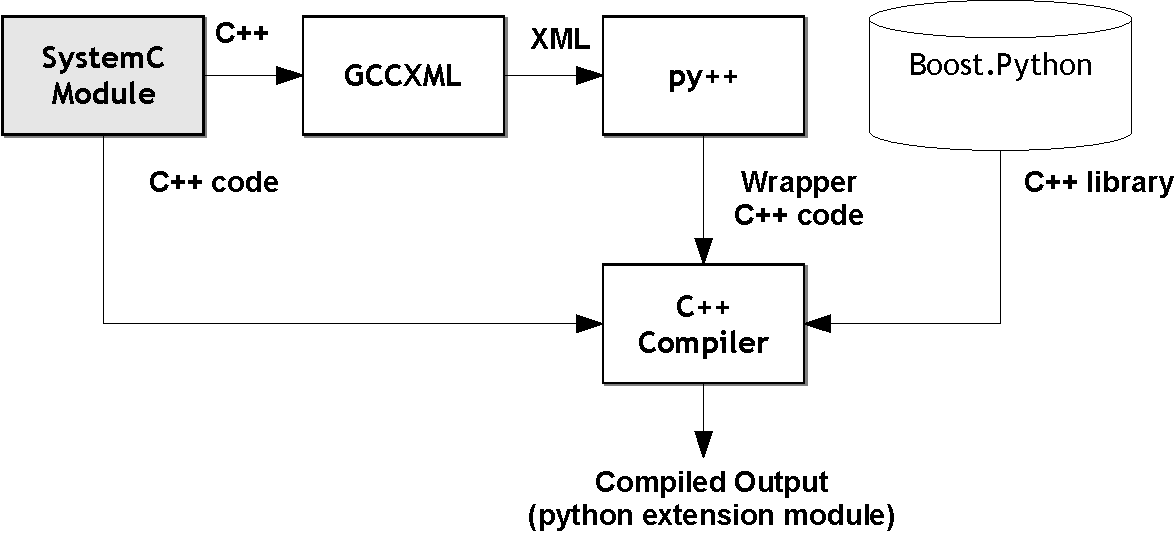
\includegraphics[width=\columnwidth]{resp-wrapperflow}
\end{center}
\caption{ReSP wrapper Generation}
\label{intro:resp:wrapper}
\end{figure}
\indent Each header file is parsed using GCCXML, a tool that provides an XML description of GCC abstract syntax tree (i.e. GCCXML produces an XML file containing the description of the classes, methods, etc. of the cpp source files; for example, for each class, the XML file contains the class name, the list of its attributes, the list of methods, etc.). The resulting XML description
is manipulated to select all the parts that need to be exported (i.e. made visible to Python), and then the OpenSource tool \texttt{py++} is used to generate Python wrapping code that uses the \texttt{Boost.Python} library. The advantage of Boost.Python and py++ over alternative tools like \texttt{SWIG} (used by most other works) is that it guarantees access to all C++ declarations, even private or protected ones, through the generation of appropriate class wrappers. The Python interpreter can load the extensions generated by the ReSP flow, and have full access to the C++, and therefore SystemC, classes contained in the exported module. Another feature of the ReSP flow is that IP documentation is automatically extracted from the SystemC source code, and inserted in
the Python wrapper. Python self-documentation features are then used to display such documentation through the User Interface.

\section{Document Outline}
\paragraph\indent This guide will show how to use the ReSP simulation platform in order to describe, simulate and analyze simple hardware architectures while running standard pieces of software cross-compiled for the specific platforms. This Chapter introduced the main idea behind this simulation platform. Starting from Chapter~\ref{install} the user will be taught how to install the tool; then, on Chapter~\ref{general} the basic use of the platform will be described and shown through some practical examples; afterwards, Chapters~\ref{reconfigurable} and~\ref{fault} will introduce some specific uses of the simulation platform while dealing with reconfigurable components and fault analysis; finally, Chapter~\ref{describe} is going to offer the basis for the development of new hardware components inside the ReSP simulation platform.


\chapter{Installing the tool}
\label{install}
\paragraph\indent This chapter contains the instructions on how to download, configure and compile the simulation platform sources. Moreover, it provides some workarounds for the users that want to directly use the platform without spending too much time worrying about the installation. 

\section{System Requirements}
\label{install:requirements}
\paragraph\indent ReSP works only on Linux systems. The simulator has been mainly developed using the Ubuntu distribution (for which some scripts for the automatic installation are provided, as discussed later in section~\ref{install:ubuntu}), and it has been tested also on several others Linux distributions such as OpenSuse 11 or on the Debian unstable release (\emph{sid}). Both the 32 and 64-bit architectures are supported; do note that SystemC experiences lower performance on 64-bit machines. This distribution of ReSP is supposed to work even on MacOSX systems, however this feature has not been tested yet, and it is not planned to test it in the future; the identification of the steps required is left to the user willing to use ReSP in such environment. Currently, it is excluded any support for Windows systems.\\
\indent The compilation process of ReSP is the most demanding operation in terms of memory and computational resources; after the compilation, however, the execution of ReSP has less strict requirements. Any machine with the following specifications is able to run this tool:
\begin{itemize}
  \item Any x86 or x86-64 compatible processor (at least a Core2Duo @ 1.66 GHz or equivalent is highly recommended);
  \item 512 MB of RAM (at least 1 GB is highly recommended);
  \item 1 GB of free space on the hard drive;
\end{itemize}

\section{Downloading the source code}
\label{install:download}
\paragraph\indent ReSP project is hosted on Google Code at the address \url{http://code.google.com/p/resp-sim/}. The source code of the project is managed through the \texttt{subversion} system (\url{http://subversion.apache.org/}). Thus, once installed the \texttt{subversion} (or shortly \texttt{svn}) client, it is possible to download the source code in the desired directory \texttt{my-resp} by executing the following command in a console:
\begin{verbatim}
  svn checkout http://resp-sim.googlecode.com/svn/trunk/ my-resp
\end{verbatim}

\section{Building and Installation Instruction}
\label{install:instr}
\paragraph\indent ReSP uses \texttt{waf} (\url{http://code.google.com/p/waf}) as build system; from a user point of view it is similar to the usual autotools based project: first there is a configuration step, then the compilation and, finally, the installation. Before the configuration step, however, some pre-requisites should be installed on the system; they are listed in the following sections.

\subsection{Required Libraries and Tools}
\paragraph\indent The following list contains all the tools and libraries required by ReSP. Do note that they should be installed following the list order, since there are some dependencies among the tools/libraries.
\begin{itemize}
  \item \textbf{waf} - the build system used by ReSP; a version of the \texttt{waf} tool is already available in the ReSP main folder, however the user may prefer a system wide installation with the most recent version of \texttt{waf} released on (\url{http://code.google.com/p/waf}).
  \item \textbf{GCC}, \textbf{G++} and \textbf{CPP} \textless= 4.2 - the older versions of the GNU compilers are required by the GCCXML tool. They are available in all Linux distributions.
  \item \textbf{Python} - a quick and easy interpreted language. Versions ranging from 2.4 to 2.6 are currently supported, however Python 2.6 works only if the latest boost libraries are installed (\textgreater= 1.42). It is available in most of Linux distributions; do note that the development version of this package is needed. Otherwise, it can be downloaded from \url{http://www.python.org/}. 
  \item \textbf{libboost} - widely used set of C++ libraries, downloadable from \url{http://www.boost.org}. Do note that they are available in most of Linux distributions. If downloaded from the official web site, installation instructions are present on that website. Actually not all the boost libraries are needed: Boost.Python, Boost.Threads, Boost.Graph, Boost.RegEx, Boost.Unit\_Test\_Framework, and Boost.Program\_Options should be enough; anyway we suggest to install the whole collection of Boost libraries. 
  \item \textbf{GCCXML} - the purpose of the GCCXML extension is to generate an XML description of a C++ program from GCC's internal representation. For this project it is required to have at least version 0.9. Since there are different 0.9 releases, we suggest you go to website \url{http://www.gccxml.org/HTML/Download.html} and get the latest version from the CVS repository. Some Linux distributions (e.g.: Ubuntu) provide it in their package repository.
  \item \textbf{pygccxml} and \textbf{py++} - tools required to navigate and expose C++ classes in a Python environment. At least version 1.5 is required. Such version has not been released yet as a separate download, but it is available on the development SVN repository (at least revision 1740 is required). Once downloaded, just run \texttt{python setup.py install} (with administrator rights) in both folders \texttt{pyplusplus\_dev} and \texttt{pygccxml\_dev}, containing the development version of the two tools.
  \item \textbf{SystemC} - downloadable from \url{http://www.systemc.org}, it is the de-facto standard in the high abstraction level modeling and simulation of hardware modules. Instructions on how to install it are contained in the SystemC package itself. Note that on 64 bits architectures you might need to patch the sources; you may do this using the patch file and the instructions contained in \texttt{ext/systemc} sub-folder of the ReSP downloaded directory (you should see if you need to patch them if you get an error during the ReSP configuration process).
  \item \textbf{TLM 2.0} - downloadable from \url{http://www.systemc.org}, it is used to model the hardware modules and, in particular, their interconnections with the Transaction Level Modeling (TLM) approach.
  \item \textbf{BFD}~\cite{binary_binutils} - tool included in the \texttt{binutils} collection, it is used to read and parse the application software which is going to be executed on the processors. It is available in all Linux distributions; do note that the development version of this package is needed. On 64 bits architectures you might need to manually download binutils sources and patch them according to the instructions in \texttt{ext/binutils} sub-folder of the ReSP downloaded directory (you should see if you need to patch them if you get an error during the ReSP configuration process).
  \item \textbf{TRAP}~\cite{fossati_trap} - a library for the description of Instruction Set Simulators, dowloadable from the SVN repository at \url{http://code.google.com/p/trap-gen/}. Do not use the archive in the downloads since it is usually not updated. The installation of these libraries is described on the Wiki page of the project (\url{http://code.google.com/p/trap-gen/wiki/Setup}) and is somewhat similar to the one of ReSP.
\end{itemize}
\indent There are also optional libraries which, if present, enhance ReSP's capabilities:
\begin{itemize}
  \item \textbf{graphviz} - necessary to show the architecture graph. It is available in most of Linux distributions or it can be downloaded from \url{http://www.graphviz.org/}.
  \item \textbf{sigc++2.0} - available in the packet manager of your distribution (whichever you are using), it is necessary in case you also need to install the MOMH library.
  \item \textbf{MOMH} - a library necessary to enable the framework for automatic design space exploration. Instructions on how to download it are available at \url{http://home.gna.org/momh/}. The library can be downloaded also from \url{http://code.google.com/p/resp-sim/downloads/list}
\end{itemize}

\subsection{Configuration and Compilation}
\paragraph\indent Once installed all required tools and libraries, it is possible to configure and compile the simulator; as already stressed, the \texttt{waf} compilation chain is used. The \texttt{./waf configure} command can be executed in the main ReSP directory for the configure step; all the configuration options which can be passed to the \texttt{./waf configure} command are hereby listed:
\begin{itemize}
  \item \textit{--with-systemc=SYSC\_FOLDER} specifies the location of the SystemC 2.2 library. It is mandatory to specify such option.
  \item \textit{--with-tlm=TLM\_FOLDER} specifies the location of the TLM 2.0 library. It is mandatory to specify such option.
  \item \textit{--with-trap=TRAP\_FOLDER} specifies the location of the TRAP runtime libraries and headers. It must be specified if TRAP was installed in a custom folder, otherwise the configuration is able to automatically detect the installation in the standard system path.
  \item \textit{--boost-includes=BOOST\_HEAD\_FOLDER} specifies the location of the header files of the boost libraries. It has to be specified in case the includes are not installed in a standard system path.
  \item \textit{--boost-libs=BOOST\_LIB\_FOLDER} specifies the location of the library files of the boost libraries. It has to be specified in case the libraries are not installed in a standard system path. Do note that if you manually installed the boost libraries, you probably need to update the environmental variable \texttt{LD\_LIBRARY\_PATH} specifying the path of the boost libraries, otherwise you will obtatin some runtime errors while loading the shared libraries.
  \item \textit{--with-bfd=BFD\_FOLDER} specifies the location of the BFD library. It has to be specified in case \texttt{libbfd} is not installed in a standard system path.
\end{itemize}

\paragraph\indent After the configuration successfully ends, compilation can be started with the plain \texttt{./waf} command. Now, it is possible to start the simulator by means of the \texttt{./startSim.sh} script (simulation use will be explained in the next chapter).
Further details on the configuration and compilation options can be obtained by issuing \texttt{./waf --help}.

\subsection{Cross-compiled Software}
\paragraph\indent In order to run pieces of software on the Instruction Set Simulators (ISS), it is required to compile them using the cross-compilers specific for the used ISS. Do note that in order to enable all the Trap ISS features, and in particular the OS emulation, the standard crosscompilers have been patched; the crosscompilers for the ISS currently included in ReSP can be downloaded from \url{http://code.google.com/p/resp-sim/downloads/list}  or from the project SFTP server (see references in Section~\ref{install:VM}). Once the compilers are decompressed, the applications can be properly cross-compiled using the \texttt{[arch]-elf-[gcc/g++]} tool in the bin directory of the desired architecture. For the proper compilation of the applications making calls to operating system routines, the \texttt{-specs=osemu.specs} command line option has to be passed to the compiler. ReSP also provides a full set of example and benchmarks programs that are stored in the \texttt{software} subdirectory: the compilation of these applications can be automatically performed using the \texttt{waf} tool inside the \texttt{software} subdirectory. The configuration options which can be passed to the \texttt{./waf configure} command are:
\begin{itemize}
  \item \textit{--arm-compiler=/PATH\_TO/cross-compilers/arm/} specifies the location of the ARM cross-compiler.
  \item \textit{--sparc-compiler=/PATH\_TO/cross-compilers/sparc/} specifies the location of the SPARC cross-compiler for the LEON ISSs.
\end{itemize}
\indent After the configuration successfully ends, compilation can be started with the usual \texttt{./waf} command.

\subsection{Platform Testing}
\paragraph\indent To check the correct compilation of the entire platform, the command \texttt{./waf -C} can be issued in ReSP main directory. This command will launch the simulation of some architectures using some application contained into the software folder, thus even the software should be cross-compiled before launching the test.

\section{Simplified installation for Ubuntu OS}
\label{install:ubuntu}
\paragraph\indent The latest two releases of Ubuntu (9.10 Karmic Koala and 10.04 Lucid Lynx) have all the proper versions of dependent software in their package repository. We provide a single script to automatically collect all the dependent software and perform its installation. Prerequisites:
\begin{itemize}
  \item You need to have administrator rights to perform the automatic installation. The script uses the standard \texttt{sudo} command, and will most likely require the input of your password only once.
  \item You must have an active Internet connection to download the required packages.
\end{itemize}
\paragraph\indent The installation is started by simply running the script \texttt{lucid-install.sh} from the root of the ReSP tree: \texttt{sudo sh ./lucid-install.sh}. Choose the 32 or 64 bit installer according to the base architecture of your OS (you can obtain it by issuing the command \texttt{uname -m} in a teminal).

\section{Virtual Machine}
\label{install:VM}
\paragraph\indent A Virtual Machine running with VirtualBox v3.0 is distributed on the project SFTP server with a version of ReSP already configured and compiled. The user can simply download it and directly start to use the tool. The project SFTP server is available at the following address:
\begin{verbatim}
  pc121-202.elet.polimi.it:22
\end{verbatim}
In order to download the contents, you'll have to access the machine with a specific user; its credentials are:
\begin{verbatim}
  Username:  downloader
  Password:  getVM
\end{verbatim}
The virtual machine runs an Ubuntu operating system; the credentails to login are:
\begin{verbatim}
  Username:  resp
  Password:  resp
\end{verbatim}
ReSP is installed in the \texttt{home} directory. 
After the download of the machine it is suggested to check for any updates on the project repository and to recompile ReSP. To check for updates execute \texttt{svn up} from a console in the \texttt{resp-sim} folder. In case of updates, execute \texttt{./waf} command both in the \texttt{resp-sim} and \texttt{resp-sim/software} folders. Partial recompilation may fail in some particular scenarios causing compile-time or run-time errors; in this situations, it is necessary to execute the following commands in the main project folder:
\begin{enumerate}
 \item \texttt{./waf distclean}
 \item \texttt{./waf configure --with-systemc=External\_tools/systemc-2.2.0 -with-tlm=External\_tools/TLM2}
 \item \texttt{./waf}
\end{enumerate}



\chapter{General Usage}
\label{general}
\paragraph\indent This chapter describes the general use of the simulation tool. The first section will give a general introduction to the directory structure inside the tool source code, while the second part is going to give an hands-on description of the capabilities of ReSP.

\section{Structure of Folders}
\paragraph\indent In order to use ReSP  and to exploit its advanced features it is very important  to know how the source code of the simulator is organized. 
Here the overall structure of the project folders is presented. Do note that there may be further folders not documented here; such folders contain not maintained code or additional features still under development.
\label{general:folders}
\begin{description}
  \item[architectures] contains the template files which describe various architectures: these files use the components of the simulator (processors, memories, etc.) to create complete architectures. The only way of specifying architectures is through Python scripts which contain the commands that the user would manually run from console in order to create the same architecture. (\texttt{base} sub-folder contains not maintained code).
  \item[components] contains the component models available to be used inside ReSP:
  \begin{description}
    \item[interconnect] contains various kinds of interconnection layers, such as buses and NOCs; so far we have an arbitrated bus (a modified version of the \texttt{pv\_router} in TLM 2.0 examples) and a simple NOC which, so far, is specified at transaction level only (no low-level packet inspection).
    \item[memories] contains a simple slave memory without controllers and two versions of a cache memory: an incoherent one, which is not recommended for multi-core architectures, and a coherent one, which uses a directory component to assign unique privileges to concurrent cache systems.
    \item[processors] contains the Instruction Set Simulators, obtained through the TRAP automatic generator. So far, only the functional loosely timed version of an ARM7TDMI, an ARM9TDMI and a LEON3 processor have been defined.
    \item[reconfigurable] contains the various models defined for the simulation of dynamically reconfigurable architectures, as described in Chapter~\ref{reconfigurable}.
    \item[reliability] contains various kinds of components used for the fault injection campaigns (further details are provided in Chapter~\ref{fault}).
    \item[testComponents] contains some simple examples of SystemC modules working as master and slave. The content of this folder will be used as a basic guide in the next part of this chapter.
  \end{description}
  \item[dse] contains the source code for a design space exploration tool (still under development).
  \item[ext] contains the patches required by binutils and SystemC on 64-bit systems.
  \item[lib] contains some external libraries used by ReSP; in particular, a dynamic version of the binutils and SystemC libaries is rebuilt at compilation time using some specific code files.
  \item[software] contains software which is executed and simulated inside the platform (cross-compilers are needed inside this folder):
  \begin{description}
    \item[apps] contains some sample application programs (such as \texttt{ffmpeg}).
    \item[lib] contains the stub required to compile programs using OpenMP and pthreads.
    \item[simple\_benchmarks] contains some real life applications used to test the general ReSP behavior.
    \item[suites] contains collections of test applications, such as the one contained in the OpenMP Source Code Repository.
    \item[test\_code] contains some specific chunks of code used to perform basic tests on the different ReSP functionalities.
  \end{description}
  \item[src] contains the simulator source files (i.e. the simulator core); these are all the files necessary for connecting the components, instantiate them, keeping track of the connections, starting and pausing simulation\ldots
  \begin{description}
    \item[bfdFrontend and \textasteriskcentered\_wrapper] contain the wrappers around SystemC which makes SystemC objects visible from Python.
    \item[cm] contains the Configuration Manager used by the OS emulation layer to manage multi-threading and concurrency.
    \item[controller] contains the files of the simulation controller, which allows to start, pause and stop the SystemC kernel.
    \item[fi] contains the Fault Injector tool used in Chapter~\ref{fault}.
    \item[hci] contains the user interfaces; the only used interface present here is the console, a command line user interface. A client-server version of the interface based on sockets is also available.
    \item[loader] contains the tool responsible for loading an application in the system program memory.
    \item[manager] contains the class that manages the components of ReSP and takes care of connecting them.
    \item[power] contains a stub of a power analysis tool (still under development).
    \item[utils] contains a series of utility functions used throughout the whole system.
  \end{description}
  \item[tools] contains the tools which may be useful to ReSP, but which are not necessary:
  \begin{description}
    \item[client] is a simple command line client used to remotely command the ReSP simulator (not maintained).
    \item[waf] contains compilation related tools: this includes the wrapper generator (for automatically creating Python wrappers around C++ objects), the doxygen documentation extractor, etc.
  \end{description}
\end{description}

\section{Using ReSP}
\label{general:using}
%\paragraph\indent How to use the ReSP simulator is presented here. First, the basic simulation commands are described. Then, the specification of a complex architecture using the most of the ReSP features is commented in details; the user can start from this specification to describe his custom architectures. Finally, the sevaral simulation modes that can be executed by speci

%\subsection{Basic Simulation Commands}
\paragraph\indent The simulator is started by executing the \texttt{./startSim.sh} command into the ReSP main folder. The simulator console that shows up is a slightly modified Python Shell; thus, it is possible to execute all the Python commands plus further specific commands defined in the simulator. For this reason, to be able to use ReSP, it is necessary to have a basic knowledge of the Python language. The console supports the command autocompletion by means of the \texttt{TAB} key, the browsing of the command history by means of the arrow keys and the search on the command history by means of the key combination \texttt{CTRL+R}.

\indent In order to instantiate a SystemC component, it is necessary to call the specific constructor and to assign the returned object to a reference. For instance, the following two commands instantiate a \texttt{testMaster} component and a \texttt{testSlave} one:

\scriptsize
\begin{verbatim}
  instMaster = testMaster_wrapper.testMaster('master')
  instSlave = testSlave_wrapper.testSlave('slave')
\end{verbatim}
\normalsize

Do note that each component class contained in the ReSP repository is included in a module during the generation of Python wrappers for the C++ code. For instance, the \texttt{testMaster} component class is included in the \texttt{testMaster\_wrapper} module. A full list of components and their wrappers can be obtained by pushing the Python \texttt{dir()} command, or by invoking the \texttt{listComponents()} command, or by browsing the \texttt{components} folder.

\indent Since all the C++ stuff is fully integrated into the Python Shell, it can be completely managed as any other Python object. Thus, for instance, issuing the \texttt{dir(instMaster)} command returns the list of public attributes and methods contained in that specific object; in this way, it is possible to know that, for example, the component has an attribute \texttt{count} and an initiator TLM port named \texttt{initSocket}. In addition, it is also possible to access the attributes and launch the methods. The next lines, issued in the console, show how it is possible to read and to write the content of the \texttt{count} attribute:

\scriptsize
\begin{verbatim}
  print str(instMaster.count)
  instMaster.count = 4
\end{verbatim}
\normalsize

\indent The instantiated components can be interconnected by means of the \linebreak \texttt{connectPorts} command: this command acts on the TLM ports declared inside the SystemC components. The parameters required by the command are: a reference of the master component, a reference to the TLM initiator port of the master component, a reference to the slave component and a reference to the TLM target port of the slave component. For example, to interconnect the two components previously instantiated, the following command needs to be executed:

\scriptsize
\begin{verbatim}
  connectPorts(instMaster, instMaster.initSocket, instSlave, instSlave.targetSocket)
\end{verbatim}
\normalsize

Please remember that the explicit call of the \texttt{bind} method exported by the TLM interface is deprecated, because it doesn't allow the simulator to keep track of the specified connections. After the connection, it is possible to show a graphical representation of the intantiated architecture by issuing the \texttt{showArchitecture()} command. It is worth noting that all the commands for the management of the architecture (\texttt{connectPorts}, \texttt{showArchitecture()} and many others) are defined as methods of the \texttt{manager} object always present in the ReSP console; refer to that \texttt{manager} for further features for the architecture management.

\indent Now it is time to start the simulation; four main commands are used to control the SystemC simulation kernel:
\begin{itemize}
  \item \texttt{run\_simulation(n)}: it is used to start (or resume) simulation for \emph{n} nanoseconds. If \emph{n} is omitted the simulation runs until the end. Do note that the execution of the command is non-blocking: the command releases immediately the console prompt even if the simulation is still running. The simulation will halt after the execution of the specified time period or until the end of the simulation is reached (some component has called the SystemC \texttt{sc\_stop()} method). In the first case, a specific message (\texttt{Simulation Paused!}) is shown at the end of the simulated time period; in the latter, the final simulation statistics are displayed (see the last part of Section~\ref{general:arch}).
  \item \texttt{pause\_simulation()}: pauses the simulation. It can be issued also with the \texttt{CTRL+C} key combination. It can then be resumed with the \texttt{run\_simulation(n)} command.
  \item \texttt{stop\_simulation()}: stops the simulation (it actually calls the \texttt{sc\_stop} method). After this method is called, it is not possible to resume the current execution and a simulator reset is necessary to perform another simulation. Do note that it is not allowed to use \texttt{stop\_simulation()} command in an architecture file (it is allowed in case of batch simulation; refer to the next section).
  \item \texttt{reset()}: stops the simulation, if running, and deletes all the stuff instantiated for the current simulation. After a reset, it is possible to instantiate a new architecture and to start a new simulation. 
\end{itemize}

\indent Do note, if an exception is thrown during the simulation by a SystemC component after a critical error, the simulator cannot be forced to continue or restarted any more; however, it is still possible to use the console, and thus, if necessary, to analyze the components' state in order to understand the causes of the error. In order to execute another simulation, ReSP needs to be quit.

\indent The architecture to be simulated can also be described in a Python script file. In this case, the architecture can be loaded by issuing the \texttt{load\_architecture()} command, requiring as parameter the name (and the path) of the file to be loaded. For instance, the architecture previously instantiated is also specified in the \texttt{architectures/test/test\_arch.py} file, and can be loaded by issuing the following command:

\scriptsize
\begin{verbatim}
  load_architecture('architectures/test/test_arch.py')
\end{verbatim}
\normalsize

Since the \texttt{run\_simulation(n)} command is non-blocking, it is forbidden to specify any other command in the architecture file after the \texttt{run\_simulation(n)} command; such command would be executed immediately after the beginning of the simulation, resulting into an incorrect behavior. To reload the same architecture after a \texttt{reset()}, it is possible to use the \texttt{reload\_architecture()} command.

\indent It is possible to obtain further information on the available commands by issuing \texttt{show\_commands()} or \texttt{dir()} on the console. At the end, the simulator can be quit by using the \texttt{exit()} command or the \texttt{CTRL+D} shortcut.

\section{Specifying a Complex Architecture}
\label{general:arch}
\paragraph\indent This section analyzes an example specification for a complex multi-processor architecture. The entire example is contained in the \texttt{architectures/ test/test\_coherent\_caches.py} file.

\indent The description starts with the assignment of the several parameters of the hardware components such as the processor frequency and type, the characteristics of the memory system, and the information about the interconnection layer. All these parameters will be used later during the components' instantiation and setup.

\scriptsize
\begin{verbatim}
  ###### GENERAL PARAMETERS #####
  PROCESSOR_FREQUENCY = 1000        # MHz
  PROCESSOR_NUMBER  = 4             #
  try:
    PROCESSOR_NAMESPACE
  except:
    PROCESSOR_NAMESPACE = arm7tdmi_funcLT_wrapper.Processor_arm7tdmi_funclt

  # Memory/bus
  MEMORY_SIZE        = 32              # MBytes
  MEM_LATENCY        = 10.0            # ns
  BUS_ACTIVE         = True
  BUS_LATENCY        = 10.0            # ns
  DATA_CACHE_ACTIVE  = True
  INSTR_CACHE_ACTIVE = True
  CACHE_SIZE         = 8               # MBytes
  CACHE_BLOCK_SIZE   = 32              # words
  CACHE_WAYS         = 8
  CACHE_REM_POLICY   = CacheLT32.LRU
  CACHE_WR_POLICY    = CacheLT32.BACK
  CACHE_READ_LAT     = 1.0             # ns
  CACHE_WRITE_LAT    = 1.0             # ns
  CACHE_LOAD_LAT     = 1.0             # ns
  CACHE_STORE_LAT    = 1.0             # ns
  CACHE_REMOVE_LAT   = 1.0             # ns
\end{verbatim}
\normalsize

\indent Then, the application to be run inside the simulation and its input parameters are specified (this operation can be substituted by the \texttt{--custom-parameters} command line option described in section~\ref{general:modes}). The software executable is automatically retrieved if placed into the software build directory or into the ReSP main folder.

\scriptsize
\begin{verbatim}
  # Software
  try:
    SOFTWARE
  except:
    SOFTWARE = 'c_pi'

  if SOFTWARE:
    try:
      ARGS
    except:
      ARGS = []
      ARGS.append('c_pi')

  # Find the specified software in the _build_ directory if not an absolute path
  if not SOFTWARE or not os.path.isfile(SOFTWARE):
    SOFTWARE = findInFolder(SOFTWARE, 'software/build/arm/')
    if not SOFTWARE:
        raise Exception('Unable to find program')
\end{verbatim}
\normalsize

\indent Now, the processors and the memory are instantiated and configured with the parameters specified above.

\scriptsize
\begin{verbatim}
  ###### PROCESSOR INSTANTIATION #####
  processors = []
  latency = scwrapper.sc_time(float(1000)/float(PROCESSOR_FREQUENCY),  scwrapper.SC_NS)
  for i in range(0, PROCESSOR_NUMBER):
    processors.append(PROCESSOR_NAMESPACE('processor_' + str(i), latency))

  ##### MEMORY INSTANTIATION #####
  memorySize = 1024*1024*MEMORY_SIZE
  latencyMem = scwrapper.sc_time(MEM_LATENCY, scwrapper.SC_NS)
  mem = MemoryLT32.MemoryLT32('mem', memorySize, latencyMem)
\end{verbatim}
\normalsize

\indent If required, the bus is instantiated too. Moreover, it is connected to the memory and the position of the main memory in the address space is bound to the first slot of the bus multi-initiator TLM socket. Keep in mind that the bus binding is completely positional: this first request binds a set of address to the first socket; the next one will bind another set to the second socket; \ldots; the \emph{n}-th request will bind a set of addresses to the \emph{n}-th slot of the multiple socket. So, remember to issue \texttt{addBinding} immediately after you connect a new slave component to the bus.

\scriptsize
\begin{verbatim}
  if BUS_ACTIVE:
    latencyBus = scwrapper.sc_time(BUS_LATENCY, scwrapper.SC_NS)
    bus = BusLT32.BusLT32('bus',2*PROCESSOR_NUMBER,latencyBus)
    connectPorts(bus, bus.initiatorSocket, mem, mem.targetSocket)
    # Add memory mapping
    bus.addBinding("mem",0x0,memorySize)
  else:
    raise Exception('Multi-core systems need to have an interconnection layer between\
    processors and memory')
\end{verbatim}
\normalsize

\indent If the caches are enabled, they need to be instantiated and interconnected to the other components. The model required for a multi-processor system is a distributed cache memory system with a shared directory devoted to the cache coherency management. Moreover, do note that according to the Harvard architecture, TRAP processors are provided with two ports: an instruction port and data port.

\scriptsize
\begin{verbatim}
  if DATA_CACHE_ACTIVE or INSTR_CACHE_ACTIVE:
    directory = DirectoryLT32.DirectoryLT32('dir',2*PROCESSOR_NUMBER)

  ##### CACHE, BUS, AND MEMORY CONNECTIONS #####
  dataCaches = []
  instrCaches = []
  for i in range(0, PROCESSOR_NUMBER):
    if DATA_CACHE_ACTIVE:
      dataCaches.append(CoherentCacheLT32.CoherentCacheLT32('dataCache_' + str(i), \
        CACHE_SIZE*1024*1024, memorySize, CACHE_WAYS, CACHE_BLOCK_SIZE, \
        CACHE_REM_POLICY, CACHE_WR_POLICY))
      dataCaches[i].setReadLatency(scwrapper.sc_time(CACHE_READ_LAT,scwrapper.SC_NS))
      dataCaches[i].setWriteLatency(scwrapper.sc_time(CACHE_WRITE_LAT,scwrapper.SC_NS))
      dataCaches[i].setLoadLatency(scwrapper.sc_time(CACHE_LOAD_LAT,scwrapper.SC_NS))
      dataCaches[i].setStoreLatency(scwrapper.sc_time(CACHE_STORE_LAT,scwrapper.SC_NS))
      dataCaches[i].setRemoveLatency(scwrapper.sc_time(CACHE_REMOVE_LAT,scwrapper.SC_NS))
      connectPorts(processors[i], processors[i].dataMem.initSocket, dataCaches[i], \
        dataCaches[i].targetSocket)
      connectPorts(dataCaches[i], dataCaches[i].dirInitSocket, directory, \
        directory.targetSocket)
      connectPorts(directory, directory.initSocket, dataCaches[i], \
        dataCaches[i].dirTargetSocket)
      connectPorts(dataCaches[i], dataCaches[i].initSocket, bus, bus.targetSocket)
    else:
      connectPorts(processors[i], processors[i].dataMem.initSocket, bus, \
        bus.targetSocket)

    if INSTR_CACHE_ACTIVE:
      instrCaches.append(CoherentCacheLT32.CoherentCacheLT32('instrCache_' + str(i), \
        CACHE_SIZE*1024*1024, memorySize, CACHE_WAYS, CACHE_BLOCK_SIZE, \
        CACHE_REM_POLICY, CACHE_WR_POLICY))
      instrCaches[i].setReadLatency(scwrapper.sc_time(CACHE_READ_LAT,scwrapper.SC_NS))
      instrCaches[i].setWriteLatency(scwrapper.sc_time(CACHE_WRITE_LAT,scwrapper.SC_NS))
      instrCaches[i].setLoadLatency(scwrapper.sc_time(CACHE_LOAD_LAT,scwrapper.SC_NS))
      instrCaches[i].setStoreLatency(scwrapper.sc_time(CACHE_STORE_LAT,scwrapper.SC_NS))
      instrCaches[i].setRemoveLatency(scwrapper.sc_time(CACHE_REMOVE_LAT,scwrapper.SC_NS))
      connectPorts(processors[i], processors[i].instrMem.initSocket, instrCaches[i], \
        instrCaches[i].targetSocket)
      connectPorts(instrCaches[i], instrCaches[i].dirInitSocket, directory, \
        directory.targetSocket)
      connectPorts(directory, directory.initSocket, instrCaches[i], \
        instrCaches[i].dirTargetSocket)
      connectPorts(instrCaches[i], instrCaches[i].initSocket, bus, bus.targetSocket)
    else:
      connectPorts(processors[i], processors[i].instrMem.initSocket, bus, \
        bus.targetSocket)
\end{verbatim}
\normalsize

\indent After the instantiation of the overall architecture, the software executable is loaded in the memory and the processors' interfaces are accordingly set up.

\scriptsize
\begin{verbatim}
  ##### LOAD SOFTWARE #####

  import os
  if not os.path.exists(SOFTWARE):
    raise Exception('Error, ' + str(SOFTWARE) + ' does not exists')

  loader = loader_wrapper.Loader(SOFTWARE)
  #Initialization of the processors and loading in memory of the application program
  print "Writing memory"
  loader.loadProgInMemory(mem)

  print "Setting up CPU registers"
  for i in range(0, PROCESSOR_NUMBER):
    processors[i].ENTRY_POINT = loader.getProgStart()
    processors[i].PROGRAM_LIMIT = loader.getProgDim() + loader.getDataStart()
    processors[i].PROGRAM_START = loader.getDataStart()
    processors[i].resetOp();
    # Set the processor ID
    processors[i].MP_ID.immediateWrite(i)
\end{verbatim}
\normalsize

\indent Thus, the operating system and POSIX thread concurrency emulation facilities are enabled. They are enabled by means of two tools provided in the TRAP library that need to be instantiated and registered in the processors' interfaces. A further description of these tools is given in section~\ref{general:advanced:tools}.

\scriptsize
\begin{verbatim}
  OS_EMULATION = True     # True or False

  # Now I initialize the OS emulator
  print "Setting up OS Emulation"
  tools = list()
  if OS_EMULATION:
    trapwrapper.OSEmulatorBase.set_program_args(ARGS)
    for i in range(0, PROCESSOR_NUMBER):
        curEmu = trapwrapper.OSEmulator32(processors[i].getInterface())
        curEmu.initSysCalls(SOFTWARE)
        processors[i].toolManager.addTool(curEmu)
        ##### CONCURRENCY MANAGEMENT #####
        concurrentEmu = cm_wrapper.ConcurrencyEmulator32(processors[i].getInterface(), \
            memorySize)
        concurrentEmu.initSysCalls(SOFTWARE,True)
        processors[i].toolManager.addTool(concurrentEmu)
        tools.append(curEmu)
        tools.append(concurrentEmu)
    # OpenMP Support
    trapwrapper.OSEmulatorBase.set_environ('OMP_NUM_THREADS', str(PROCESSOR_NUMBER)) 
\end{verbatim}
\normalsize

\indent The redefinition of the \texttt{statsPrinter()} function allows to customize the statistics printed at the end of the simulation:

\scriptsize
\begin{verbatim}
  # Modified stats auto-printer
  def statsPrinter():
    print '\x1b[34m\x1b[1mReal Elapsed Time (seconds):\x1b[0m'
    print '\x1b[31m' + str(controller.print_real_time()) + '\x1b[0m'
    print '\x1b[34m\x1b[1mSimulated Elapsed Time (nano-seconds):\x1b[0m'
    print '\x1b[31m' + str(controller.get_simulated_time()) + '\x1b[0m'
\end{verbatim}
\normalsize

\indent Finally, the simulation is executed. Remember, it is forbidden to put any other command after the \texttt{run\_simulation()} into the architecture files. Further commands have to be issued directly into the ReSP console.

\scriptsize
\begin{verbatim}
  # We can finally run the simulation
  run_simulation()
\end{verbatim}
\normalsize

\section{Command Line Options and Execution Modes}
\label{general:modes}
\paragraph\indent When launching ReSP, you can specify several command line options to be used; they offer different advanced simulation modes. Here is a list of the most relevant options supported by \texttt{startSim.sh}:
\begin{itemize}
  \item \texttt{--architecture ARCHITECTURE.py} or \texttt{-a ARCHITECTURE.py}: automatically loads the specified architecture inside the simulator (the relative path of the architecture file should be specified). For instance, to load architecture \texttt{architectures/test\_arch.py} you should issue the following command into your system shell:
  \begin{verbatim}
  ./startSim.sh -a architectures/test_arch.py
  \end{verbatim}
  \item \texttt{--silent}: executes the simulation in silent mode. This means that no interactive console is fired-up and the simulator exits as soon as the simulation is ended. In silent mode the \texttt{run\_simulation()} command is blocking and the \texttt{pause\_simulation()} and few other commands specified lated are disabled. This option can be specified only in conjunction with \texttt{-a} option. After loading the architecture the simulation is completely executed. If it is desired to issue specific commands, to inspect the components, or to somehow modify the execution flow, you should include the specific instructions inside the architecture file or in a batch file (refer to the next option), since the simulation process cannot be interrupted by any user interaction.
  \item \texttt{--batch BATCH\_COMMANDS.py} or \texttt{-b BATCH\_COMMANDS.py}: executes a Python script containing some batch actions to be executed after the architecture file is loaded. This option can be specified only in conjunction with \texttt{-a} and \texttt{--silent} options.
  \item \texttt{--custom-parameters COMMAND} or \texttt{-p COMMAND}: a Python instruction can be used to set up some custom parameters before the architecture file is loaded. The syntax of the command must be in the form \texttt{PAR1=VALUE1;PAR2=VALUE2} (i.e. without spaces). For instance it is possible to specify the name of the software to be loaded in the test architecture of the ARM7 processor by means of the following command:
  \begin{verbatim}
  ./startSim.sh -a architectures/test/test_arm7.py 
    -p SOFTWARE='des';ARGS=[]
  \end{verbatim}
  Do note that it is necessary to specify the escape character \textbackslash before the character \texttt{'}. The options accepts also the name of a file containing the several custom parameters. Moreover, after a reset of the simulator, the custom parameters are automatically reloaded with the \texttt{reload\_architecture()} command. If not required, it is necessary to pass a \texttt{False} value as parameter to that command.
  \item \texttt{--server SERVER\_PORT} or \texttt{-s SERVER\_PORT}: starts ReSP in server mode. The port on which the server listens for connection requests has to be specified. Currently a simple command line client is provided; it can be launched by running the \texttt{python src/hci/remote\_console.py} command (\texttt{--help} shows the available command line options).
  \item \texttt{--help} or \texttt{-h}: shows all the supported command line parameters.
\end{itemize}

\section{Advanced Features}
\label{general:advanced}
\paragraph\indent Besides the basic aspects described in the previous sections of this chapter, ReSP provides advanced features offering the capability to implement additional tools for the simulation and analysis of complex multiprocessor systems. Some of these capabilities are quickly introduced in the following sections; for the users interested in a more detailed description of these advanced features, it is suggested an analysis of the commented code of the simulator.

\subsection{SystemC Callbacks}
\label{general:advanced:breakpoints}
\paragraph\indent In ReSP, the basic SystemC simulation kernel has been enhanced by means of an advanced simulation controller that offers also the possibility to manage specific callback functions registered on some particular event. Thus, when the event is triggered, the registered callbacks are executed. The simulation controller supports four different types of callbacks:
\begin{itemize}
\item \texttt{EosCallback}: they are triggered at the end of the simulation, when the \texttt{sc\_stop()} function is called.
\item \texttt{PauseCallback}: they are triggered when the simulation enters in the pause state. They are supported only in the interactive simulation mode.  
\item \texttt{ErrorCallback}: they are triggered when a simulation error occurs and some component has thrown a C++ exception.
\item \texttt{DeltaCallback}: they are triggered after each simulation delta cycle.
\end{itemize}

\indent Thus, it is possible to implement new specific analysis tools by using the SystemC callbacks. The desired callback is implemented by extending the corresponding basic callback class, defined in \texttt{src/controller/callback.hpp} file. In particular, each basic class contains the constructor and the destructor used to set-up and tear down the callback, and a functor that is called on the event occurrence. The new callback class can be implemented both in Python and in C++: in the first case it is enough to import the module containing the class in the ReSP console; in the second case, the C++ class needs to be hooked to the compilation process (refer to Chapter \ref{describe} for further details).

\indent Let's consider an example for explaining how to define and use new callbacks. The \texttt{src/controller/breakpoints.py} file defines a dummy breakpoint mechanism offering the possibility to pause the simulation when a specified component attribute assumes a specified value. The mechanism implemented in that file makes use of a new callback \texttt{GenericBreakpoint} that is obtained as an extension of the \texttt{DeltaCallback}. In particular, the \texttt{GenericBreakpoint} class constructor requires the reference to the component object, the name of the attribute to be monitored and the object representing the condition to be evaluated; this last one is based on a set of comparator classes defined in the same file.

\indent The file contains also the \texttt{register\_breakpoint()} function that instantiates the callback and registers it in the controller; it is performed by means of the following two instructions:

\scriptsize
\begin{verbatim}
  gb = GenericBreakpoint( object, attribute, checker )
  sc_controller_wrapper.registerDeltaCallback( gb )
\end{verbatim}
\normalsize

\indent Do note that every callback instantiated in the Python console has always to be assigned to a Python reference; otherwise, the Python garbage collector will delete the object and it will cause a segmentation fault at the subsequent execution of the callback. For this reason, in the source file, all \texttt{GenericBreakpoint} objects are stored in the \texttt{breaks} list. 

\indent An example of how to use the breakpoints is shown in the following set of instructions that should be issued directly in the ReSP console:

\scriptsize
\begin{verbatim}
  load_architecture('architectures/test/test_arch.py')
  import breakpoints
  condition = breakpoints.equals(5)
  breakpoints.register_breakpoint(instMaster,'count',condition)
  run_simulation()
\end{verbatim}
\normalsize

This example executes a simple system based on the two test master and slave components; a breakpoint is set to pause the simulation after the master has sent five characters.
The example is also contained in the \texttt{architectures/test/test\_breakpoints.py} architecture file.

\indent Another example of use of the callback is contained in the \texttt{src/print\_stats.py} file where the mechanism for printing final simulation statistics is defined by extending the \texttt{EosCallback} class. This special callback is automatically registered by the tool in the \texttt{src/respkernel.py} file.\\
\indent You should always keep in mind that the implementation of \texttt{DeltaCallback} in Python causes a dramatic degradation of the performance since the execution of interpreted scripting code is considerably slower than C++ compiled one.

\subsection{TRAP Tools}
\label{general:advanced:tools}
\paragraph\indent A callback mechanism similar to the one introduced in the last section is useful also for a different purpose: using the features introduced by the BFD tool, it is possible to analyze the code of the simulated application and to trigger the calls to the routines executed on the ISSs generated with TRAP. Whenever one of these executions is triggered, it is possible to issue a new kind of callback, named \texttt{SyscallCB}, which could completely replace the original routine executed on the processor model. This kind of callback mechanism is implemented through some components named \emph{TRAP tools}. A tool is a particular type of class which implements a standard interface used inside the Instruction Set Simulators generated by TRAP: the most important methods required by the interface are the following:
\begin{description}
  \item[register\_syscall] has the purpose to bind a \texttt{SyscallCB} to a specific function name.
  \item[initSysCalls] requires a reference to the simulated software, where it searches and keeps trace of the position of all the routines registered through the previous method.
  \item[newIssue] is a method called by the ISSs for every instruction simulated. It requires the current Program Counter as a parameter, and if it matches the position of a registered callback, the corresponding \texttt{SyscallCB} is issued instead of the regular processor instruction.
\end{description}
\indent Furthermore, the tool constructor requires as a parameter a reference to the interface of the processor executing the code. Thanks to this reference, the \texttt{SyscallCB} becomes able to access and manipulate different resources of a processor. This is a key functionality if we want to access the parameters of the internally simulated routines.\\
\indent An example of how useful these tools can be is given by the Operating System Emulator instantiated in section~\ref{general:arch}: this emulator is able to intercept all the simulated routines belonging to the operating system level (such as open, read, write, chown, etc.), and to emulate them by issuing the corresponding routine on the host system instead of the simulator. For instance, if we want to open a file inside our simulation, the OS Emulator tool reassigns the job to the operating system layer of our Linux distribution, increasing the simulation speed for our application (there is no more need of loading a OS image inside the simulation platform). This kind of approach requires that every callback is declared with a rounded latency which is used to correctly model the time elapsed in the simulation. The following piece of code is an example of how a \texttt{SyscallCB} for emulating the \texttt{open} system call looks like:

\scriptsize
\begin{verbatim}
  template<class wordSize> class openSysCall : public SyscallCB<wordSize>{
    public:
    openSysCall(ABIIf<wordSize> &processorInstance, sc_time latency = SC_ZERO_TIME):
        SyscallCB<wordSize>(processorInstance, latency){}

    bool operator()(){
      this->processorInstance.preCall();
      //Lets get the system call arguments
      std::vector<wordSize> callArgs = this->processorInstance.readArgs():
      //Lets read the name of the file to be opened
      char pathname[256];
      for(int i = 0; i < 256; i++){
        pathname[i] = (char)this->processorInstance.readCharMem(callArgs[0] + i);
        if(pathname[i] == '\x0') break;
      }
      int flags = callArgs[1];
      OSEmulatorBase::correct_flags(flags);
      int mode = callArgs[2];
      #ifdef __GNUC__
      int ret = ::open(pathname, flags, mode);
      #else
      int ret = ::_open(pathname, flags, mode);
      #endif
      this->processorInstance.setRetVal(ret);
      this->processorInstance.returnFromCall();
      this->processorInstance.postCall();

      if(this->latency.to_double() > 0)
        wait(this->latency);

      return true;
    }
  };
\end{verbatim}
\normalsize
The latency and the processor interface are passed to the callback constructor by the \texttt{initSysCalls} method offered by the TRAP tool interface.

\indent Other examples of tools are the Concurrency Emulator, used to emulate multi-threaded applications, or the Reconfiguration Emulator introduced in~\ref{rec:regist}, used to emulate reconfigurable applications. The same routine could be intercepted by many different tools: the only condition required for this to happen is that the tool is registered inside the \texttt{toolManager} provided by every ISS. Thus, the standard sequence of commands necessary to instantiate a tool is the following:

\scriptsize
\begin{verbatim}
  tools = list()
  curEmu = myTool32(processors[i].getInterface())
  curEmu.initSysCalls(SOFTWARE)
  processors[i].toolManager.addTool(curEmu)
  tools.append(curEmu)
\end{verbatim}
\normalsize
Two important considerations should be made:
\begin{inparaenum}
  \item different processors require different instances of the same tool, and
  \item an instantiated tool should be added to a list in order to keep it alive and to avoid its elimination by the Python garbage collector.
\end{inparaenum}

\indent If the user wants to build its own tool, the suggestion is to follow the general structure given in the OS Emulator.

\chapter{Reconfigurable Hardware}
\label{reconfigurable}
\paragraph\indent This chapter will describe how to use the capabilities of ReSP in order to describe a dynamic reconfigurable system. The first section will show how to set up the ReSP environment with the reconfiguration elements; the second section will outline the two methodologies for writing hardware-implemented functions, using Python or C++ language; then, the third section is going to describe how to register these functions in order to use the reconfigurable system. The content of this chapter is just a quick introduction to the use of these components; a detailed description of how the emulation mechanism works is given in~\cite{fossati_hlm}.

\section{Setting up ReSP}
\label{rec:setup}
\paragraph\indent The elements used by the reconfiguration system are mainly two: a \textit{configuration engine}, and one (or more) \textit{eFPGAs}. The instantiation of these elements can be done directly in ReSP or, alternatively, in the architecture file, through these Python commands:

\scriptsize
\begin{verbatim}
  ...
  ##### RECONFIGURABLE COMPONENTS INSTANTIATION #####
  cE = cE_wrapper.configEngine('cE',0x0,cE_wrapper.LRU)
  cE.setRequestDelay(scwrapper.sc_time(3, scwrapper.SC_NS))
  cE.setExecDelay(scwrapper.sc_time(3, scwrapper.SC_NS))
  cE.setConfigDelay(scwrapper.sc_time(3, scwrapper.SC_NS))
  cE.setRemoveDelay(scwrapper.sc_time(3, scwrapper.SC_NS))

  #eFPGAs
  eF = []
  eF.append(eFPGA_wrapper.eFPGA('eF1',100,100,scwrapper.sc_time(1, scwrapper.SC_NS),1,1))
  eF.append(eFPGA_wrapper.eFPGA('eF2',200,200,scwrapper.sc_time(2, scwrapper.SC_NS),2,2))
  EFPGA_NUMBER = eF.__len__()
  ...
\end{verbatim}
\normalsize
A quick explanation of the characteristics of these elements:
\begin{description}
  \item[Configuration Engine] is the main element, which stores all the information of the reconfigurable system and takes care of the dynamic reconfiguration of the fabrics. It is defined by:
  \begin{itemize}
    \item a \textbf{name} ('cE' in the example);
    \item the \textbf{address} of the first location where the bitstreams are stored (we're using only fake bitstreams, so any address from any memory is a valid parameter);
    \item the \textbf{deletion algorithm} to be used when the fabrics are full (to be chosen between \textit{cE\_wrapper.FIFO}, \textit{cE\_wrapper.LRU}, and \textit{cE\_wrapper.RANDOM}).
  \end{itemize}

  \item[eFPGAs] are the reconfigurable fabrics, which are attached to (and managed by) the configuration engine. Each one of them stores information about the functions configured on it, in particular about the space occupation of these functions, in order to determine how much free space is available for new functions to be configured. They are defined by:
  \begin{itemize}
    \item a \textbf{name} ('eF\#' in the example);
    \item a \textbf{width} and an \textbf{height}, expressed in terms of basic computation units (or cells);
    \item the \textit{latency per word} \textbf{lw}, which is an \mbox{\textit{sc\_time}} parameter\footnote{Please note that the ReSP Python shell recognizes only nanoseconds as measuring unit of time, thus every value should be expressed through \textit{SC\_NS}.} indicating how much time is needed by this fabric to configure a single word;
    \item the \textit{words per area} \textbf{wa}, which is an integer number defining this fabric's density of words in a single unit of area (chosen by the user, i.e. $mm^{2}$);
    \item the \textit{cells per area} \textbf{ca}, which is an integer number defining this fabric's density of cells in a single unit of area (which should be the same used for wa, i.e. $mm^{2}$).
  \end{itemize}
\end{description}

\indent Table~\ref{rec:efpgas} shows the original characteristics of 3 families of FPGAs, and the derived parameters to be used for the instantiation of 3 devices in our reconfigurable system, one for each considered family. In particular, our eFPGAs will have a single \emph{cell per unit of area} (in order to simplify the calculations), while timing (the \emph{latency per word}) and density (\emph{words per area}, where a word corresponds to 32 bits) are calculated using specific devices for each family (listed in the \texttt{Timing\slash Density} row of the table), using the following formulae:
\begin{eqnarray*}
  WordsPerArea = \dfrac{Full Bitstream Size \times 8}{32}/Capacity\\ \\
  LatencyPerWord = \dfrac{Full Rec. Time}{Capacity}/WordsPerArea\\
\end{eqnarray*}

\indent The size parameters (\emph{Width} and \emph{Height}) are calculated in a simpler manner: given the capacity (i.e. number of basic cells) of a specific device of each family (listed in the \texttt{Space} row of the table), this number has been approximated and divided randomly into a horizontal and a vertical factor; multiplying together the horizontal factor (Width) and the vertical factor (Height) we can re-obtain the approximated number of basic cells in the device.

\begin{table}[htbp]
\caption{Some exaples of eFPGAs}
\label{rec:efpgas}
\begin{center}
  \begin{tabular}{|p{0.25\textwidth}|p{0.25\textwidth}||p{0.25\textwidth}|p{0.25\textwidth}|}
    \hline
    %\multicolumn{1}{|c|}{} & \multicolumn{1}{|c|}{} & \multicolumn{1}{|c|}{} & \multicolumn{1}{|c|}{} \\
    \small Family & \multicolumn{1}{|c|}{\large \textbf{Atmel}} &
    \multicolumn{1}{|c|}{\large \textbf{Virtex}} & \multicolumn{1}{|c|}{\large \textbf{Altera}} \\
    \hline
    \small Basic Cell & \multicolumn{1}{|c|}{\small Cell} & \multicolumn{1}{|c|}{\small Logic Cell} & \multicolumn{1}{|c|}{\small Logic Element} \\
    \small & \multicolumn{1}{|c|}{\small (4LUT-Based)} & \multicolumn{1}{|c|}{\small (4LUT-Based)} & \multicolumn{1}{|c|}{\small (4LUT-Based)} \\
    \hline
    \small Granularity & \multicolumn{1}{|c|}{\small Fine} & \multicolumn{1}{|c|}{\small Coarse} & \multicolumn{1}{|c|}{\small Coarse} \\
    \hline
    \small Timing\slash Density & \multicolumn{1}{|c|}{\textbf{AT40K05}} &
    \multicolumn{1}{|c|}{\textbf{XCV300}} & \multicolumn{1}{|c|}{\textbf{E20K100}} \\
    \hline
    \small Full Bitstream Size & \multicolumn{1}{|c|}{\small \numprint{5263} byte} &
    \multicolumn{1}{|c|}{\small \numprint{297860} byte} & \multicolumn{1}{|c|}{\small \numprint{125951} byte} \\
    \hline
    \small Full Rec. Time & \multicolumn{1}{|c|}{\small \numprint{5.263} \milli\second} &
    \multicolumn{1}{|c|}{\small \numprint{4.37} \milli\second} & \multicolumn{1}{|c|}{\small \numprint{12.3} \milli\second} \\
    \hline
    \small Rec. Clock & \multicolumn{1}{|c|}{\small 1 \mega\hertz} &
    \multicolumn{1}{|c|}{\small 50 \mega\hertz} & \multicolumn{1}{|c|}{\small 10 \mega\hertz} \\
    \hline
    \small Capacity & \multicolumn{1}{|c|}{\small \numprint{256}} &
    \multicolumn{1}{|c|}{\small \numprint{6912}} & \multicolumn{1}{|c|}{\small \numprint{4160}} \\
    \hline
    \small \emph{CellsPerArea} & \multicolumn{1}{|c|}{\small 1} & \multicolumn{1}{|c|}{\small 1} & \multicolumn{1}{|c|}{\small 1} \\
    \hline
    \small \emph{WordsPerArea} & \multicolumn{1}{|c|}{\small 5} & \multicolumn{1}{|c|}{\small 11} & \multicolumn{1}{|c|}{\small \numprint{7.5}} \\
    \hline
    \small \emph{LatencyPerWord} & \multicolumn{1}{|c|}{\small 4 \micro\second} &
    \multicolumn{1}{|c|}{\small 58 \nano\second} & \multicolumn{1}{|c|}{\small 400 \nano\second} \\
    \hline
    \small Space & \multicolumn{1}{|c|}{\textbf{AT40K40}} &
    \multicolumn{1}{|c|}{\textbf{XCV812E}} & \multicolumn{1}{|c|}{\textbf{E20K1500E}} \\
    \hline
    \small Capacity & \multicolumn{1}{|c|}{\small \numprint{2304}} &
    \multicolumn{1}{|c|}{\small \numprint{21168}} & \multicolumn{1}{|c|}{\small \numprint{51840}} \\
    \hline
    \small Approx. Capacity & \multicolumn{1}{|c|}{\small \numprint{2304}} &
    \multicolumn{1}{|c|}{\small \numprint{21000}} & \multicolumn{1}{|c|}{\small \numprint{50000}} \\
    \hline
    \small \emph{Width}$\times$\emph{Height} & \multicolumn{1}{|c|}{\small 24$\times$96} &
    \multicolumn{1}{|c|}{\small 150$\times$140} & \multicolumn{1}{|c|}{\small 250$\times$200} \\
    \hline
  \end{tabular}
\end{center}
\end{table}
\normalsize
\indent Once the components are instantiated, it is necessary to set up the connections among them; the following lines of a Python script are used for this purpose:

\scriptsize
\begin{verbatim}
  ...
  ##### RECONFIGURABLE COMPONENTS CONNECTIONS #####
  connectPorts(cE, cE.ramSocket, bus, bus.targetSocket)
  if CONFIGURE_THROUGH_ITC:
    connectPorts(cE, cE.destSocket, bus, bus.targetSocket)

  bSPosition = 1
  for i in range(0, EFPGA_NUMBER):
    connectPorts(cE, cE.initiatorSocket, eF[i], eF[i].targetSocket)
    if CONFIGURE_THROUGH_ITC:
      connectPorts(bus, bus.initiatorSocket, eF[i].bS, eF[i].bS.targetSocket)
      bus.addBinding("bS"+str(bSPosition), memorySize1+memorySize2+bSPosition, \
        memorySize1+memorySize2+bSPosition)
    else:
      connectPorts(cE, cE.destSocket, eF[i].bS, eF[i].bS.targetSocket)
    cE.bindFPGA(memorySize1+memorySize2+bSPosition)
    bSPosition = bSPosition+1
  ...
\end{verbatim}
\normalsize

\indent This whole script is based on a classic system where a simple bus and a simple memory are instantiated. The \texttt{ramSocket} on the configuration engine is a particular TLM port used to receive the bitstreams read from the memory thorugh the system bus; on the other hand, \texttt{destSocket} is another TLM port where the configuration engine forwards these bitstreams to the eFPGAs. Depending on the boolean parameter \texttt{CONFIGURE\_THROUGH\_ITC}, the user could decide if this second transfer is performed directly towards the eFPGAs, or if the bitstream has to be passed again through the system bus (or main interconnection). Then, for each eFPGA instantiated in the system, it should be drawn a direct connection between the \texttt{initiatorSocket} of the configuration engine and the \texttt{targetSocket} of the eFPGA. Furthermore, the bitstream sink of each eFPGA should be connected to the configuration engine \texttt{destSocket} or to the system main bus (still depending on the \texttt{CONFIGURE\_THROUGH\_ITC} parameter). In this last case, a special memory binding should be issued for the address assigned to the specific eFPGA bitstream sink. Finally, the same eFPGA address should be bound inside the configuration engine; please note that this binding is always required (even if the bitstream sink is directly connected to the configuration engine) and, furthermore, is completely positional: the order of the bindings should follow precisely the order in which the ports are connected (for a similar situation, see the bus connection performed in Section~\ref{general:arch}).

\section{Declaring the Hardware Functions}
\label{rec:decl}
\paragraph\indent In order to obtain a reconfigurable system, it is necessary to describe the hardware functions used on the reconfigurable fabrics; these functions are based on a small variation of the callbacks introduced in Section~\ref{general:advanced:tools} for the emulation of the system calls issued on the ISSs. ReSP gives us two options for describing such callbacks: \textit{Python} and \textit{C++}. Table~\ref{rec:decl:tabcomp} makes a performance comparison between them.

\definecolor{Green}{rgb}{0.2,0.8,0}
\definecolor{Red}{rgb}{0.8,0.2,0}
\definecolor{Orange}{rgb}{0.9,0.7,0}
\begin{table}
\caption{Python vs. C++ comparison}
\label{rec:decl:tabcomp}
\begin{center}
  \begin{tabular}{|p{0.38\textwidth}|p{0.22\textwidth}|p{0.3\textwidth}|}
    \hline
    \multicolumn{1}{|c|}{\textbf{Characteristic}} & 
    \multicolumn{1}{|c|}{\textbf{Python}} &
    \multicolumn{1}{|c|}{\textbf{C++}} \\
    \hline
    \small Describing easy algorithms &
    \small \textcolor{Green}{Ok} &
    \small \textcolor{Green}{Ok} \\
    \hline
    \small Describing complex algorithms &
    \small \textcolor{Red}{Not suitable} &
    \small \textcolor{Green}{Ok} \\
    \hline
    \small Quickness of use &
    \small \textcolor{Green}{High \linebreak (not compiled)} &
    \small \textcolor{Orange}{Medium \linebreak (requires compilation)} \\
    \hline
    \small Ease of use &
    \small \textcolor{Green}{High} &
    \small \textcolor{Orange}{Medium} \\
    \hline
  \end{tabular}
\end{center}
\end{table}
\normalsize

\subsection{Python}
\label{rec:decl:python}
\paragraph\indent Describing a function in Python is pretty simple, since it is an easier language than C++; though, Python suffers of some limitations such as, for example, the lack of C++ pointers. The function should be declared directly in ReSP or in the architecture file, and has to follow this class structure:

\scriptsize
\begin{verbatim}
  # Declare Python callbacks
  class templateCall(recEmu_wrapper.reconfCB32):
    def __init__(self, latency, w, h):
      recEmu_wrapper.reconfCB32.__init__(self, latency, w , h)
    def __call__(self, processorInstance):

      cE.executeForce('functionName', self.latency, self.width, self.height)
      cE.printSystemStatus()

      processorInstance.preCall();

      # Write here the core of the function, using the following syntax
      callArgs = processorInstance.readArgs()
      # Callback parameters can be accessed as shown in these instructions
      param1 = callArgs.__getitem__(0)
      param2 = callArgs.__getitem__(1)
      retVal = param1 + param2
      processorInstance.setRetVal(retVal);

      processorInstance.returnFromCall();
      processorInstance.postCall();
      return True
\end{verbatim}
\normalsize
The user can copy this code exactly as it is, changing only the \mbox{\textbf{functionName}} in the \mbox{\textit{confexec}} call (according to the overwritten software function), and, hopefully, the Python code in the core section.\\
\indent Some in-depth observations about this declaration:
\begin{itemize}
  \item the Python class is defined as a \textit{callback}, which extends the C++ class \textit{recEmu\_wrapper.reconfCB32}. The parameters for its constructor are the \textbf{latency} of its execution, and its dimension on the reconfigurable fabric, expressed as number of \textbf{width} and \textbf{height} cells;
  \item the \textit{executeForce} command issued to the configuration engine \textit{cE} is a signal to the component that a new reconfigurable routine is called. It will simulate the reconfiguration of the fabric (if needed) and the function invocation, by increasing the system execution time for the correct amount of units, and occupying the bus during the reconfiguration time. Alternatively, the separate \textit{configure} and \textit{execute} commands can be issued (check the \verb|configEngine.hpp| source file for further information);
  \item the \textit{printSystemStatus} command issued to \textit{cE} is optional, and shows the status of the reconfigurable system after the function configuration.
  \item instruction \textit{procInstance.return\_from\_syscall()} is responsible for suppressing the execution of the original function. If a user wants to execute in parallel both the functions (the software one on the processor and the hardware one on the eFPGA), this instruction should be removed, and the return value of the \textit{\_\_call\_\_} routine should be set to \textbf{False}; just remember that this way, both the latencies for the hardware and the software functions will be introduced.
\end{itemize}

\indent Finally, the callback should be instantiated using the following instruction, where the user should explicit the \textbf{latency}, \textbf{width} and \textbf{height} parameters:

\scriptsize
\begin{verbatim}
  templateInstance = templateCall(scwrapper.sc_time(latency, scwrapper.SC_NS),width,height)
\end{verbatim}
\normalsize

\subsection{C++}
\label{rec:decl:c++}
\paragraph\indent Using C++ allows the user to describe more complex functions, but requires to recompile the ReSP platform in order to have an executable code. The function should be declared in file \verb|reconfCallbacks.hpp| in the \verb|/components/reconfigurable/reconfEmulator/| directory, with the following structure:

\scriptsize
\begin{verbatim}
  template<class issueWidth> class __EXAMPLE__Call : public reconfCB<issueWidth>{
  private:
    configEngine* cE;
  public:
    __EXAMPLE__Call(configEngine* mycE, sc_time latency = SC_ZERO_TIME, \
        unsigned int width = 1, unsigned int height = 1):
      reconfCB<issueWidth>(latency, width, height), cE(mycE)	{}
    bool operator()(ABIIf<issueWidth> &processorInstance){

      (this->cE)->executeForce("functionName", this->latency, this->width, this->height);
      (this->cE)->printSystemStatus();

      processorInstance.preCall();

      // Write here the core of the function, using the following syntax
      std::vector< issueWidth > callArgs = processorInstance.readArgs();
      // Callback parameters can be accessed as shown in these instructions
      int param1 = callArgs[0];
      int param2 = callArgs[1];
      int retVal = param1 + param2;
      processorInstance.setRetVal(retVal);

      processorInstance.returnFromCall();
      processorInstance.postCall();
      return true;
    }
 };
\end{verbatim}
\normalsize
This is a standard class structure, the only interventions required for the user are to replace \textbf{template} as the name for the class (and obviously for the class constructor), the \mbox{\textbf{functionName}} in the \mbox{\textit{executeForce}} call (according to the overwritten software function) and hopefully the C++ code in the core section.\\
\indent Some in-depth observations about this declaration (they are similar to those made for Python):
\begin{itemize}
  \item the class is defined as a \textit{callback}, which extends the C++ class \linebreak \mbox{\textit{reconfCB\textless issueWidth\textgreater}}. The parameters for its constructor are the \textbf{latency} of its execution, and its dimension on the reconfigurable fabric, expressed as number of \textbf{width} and \textbf{height} cells;
  \item the \textit{confexec} command issued to the configuration engine pointed by \textit{this$\Rightarrow$cE} is a signal to the component that a new reconfigurable routine is called. It will simulate the reconfiguration of the fabric (if needed) and the function invocation, by increasing the system execution time for the correct amount of units, and occupying the bus during the reconfiguration time. Alternatively, the separate \textit{configure} and \textit{execute} commands can be issued (check the \verb|configEngine.hpp| source file for further information);
  \item the \textit{printSystemStatus} command issued to \textit{cE} is optional, and shows the status of the reconfigurable system after the function configuration.
  \item instruction \textit{procInstance.return\_from\_syscall()} is responsible for suppressing the execution of the original function. If a user wants to execute in parallel both the functions (the software one on the processor and the hardware one on the eFPGA), this instruction should be removed, and the return value of the \textit{operator()} routine should be set to \textbf{false}; just remember that this way, both the latencies for the hardware and the software functions will be introduced.
\end{itemize}

\indent Finally, a new registration branch should be added to the \textit{registerCppCall} routine at the end of \verb|reconfEmulator.hpp|:

\scriptsize
\begin{verbatim}
  if (funName=="functionName") {
    __EXAMPLE__Call<issueWidth> *rcb = NULL;
    rcb = new __EXAMPLE__Call<issueWidth>(cE,latency,w,h);
    if (!(this->register_call(funName, *rcb))) delete rcb;
  }
\end{verbatim}
\normalsize

Also these instructions are standard, the user should change only the \linebreak \mbox{\textbf{functionName}} and the instantiated \textbf{class name}. Perhaps, function parameters such as \textbf{latency}, \textbf{width} and \textbf{height} can be hardcoded during the definition of the new \textit{templateCall} class; please note that this action will overwrite every parameter defined in the system architecture (see Section \ref{rec:regist}).\\
\indent In order to use the C++ defined functions, ReSP needs to be recompiled with the \verb|./waf| command in the root directory.

\section{Registering the Functions}
\label{rec:regist}
\paragraph\indent Now that the callbacks are defined, they should be registered in order to be invoked every time the corresponding call is encountered during the execution. This behavior could be achieved by introducing a new tool to be attached to the ISS: this tool is known as \emph{Reconfiguration Emulator}. In multiprocessor systems, an emulator should be declared for each and every on of the ISSs; therefore, we have to cycle through all the processing elements in order to bind the emulators and, for each of them, we have to register the routines to be emulated through hardware using the \texttt{registerCppCall} and \texttt{registerPythonCall} functions offered by the reconfiguration emulator. The following Python script exemplifies this process:

\scriptsize
\begin{verbatim}
  pytCalls = list()
  # Now I initialize the Reconfiguration Emulator
  for i in range(0, PROCESSOR_NUMBER):
    recEmu = recEmu_wrapper.reconfEmulator32(processors[i].getInterface(),cE,SOFTWARE)
    processors[i].toolManager.addTool(recEmu)
    tools.append(recEmu)

    # Registration of the callbacks
    pythonCallInstance = pythonCall(scwrapper.sc_time(1, scwrapper.SC_NS),50,100)
    recEmu.registerPythonCall('PythonDefinedFunctionName', pythonCallInstance);
    pytCalls.append(pythonCallInstance)

    recEmu.registerCppCall('C++DefinedFunctionName',scwrapper.sc_time(1,scwrapper.SC_NS),50,100)
    recEmu.registerCppCall('C++DefinedFunctionName');

    print 'Registered routine calls for processor ' + str(i) + ': '
    recEmu.printRegisteredFunctions()
\end{verbatim}
\normalsize

Some notes about this piece of code:
\begin{description}
  \item[Python vs. C++] Do note that latency and dimension parameters for Python are assigned during the instantiation, while for C++ they're assigned at registration time; if they're omitted (see the second \texttt{registerCppCall} call above), standard latency is going to be 0 seconds, and standard dimension is 1x1 cells. Furthermore, while the functions defined in C++ are automatically found in the \mbox{\textit{registerCppCall}} routine (as done in Section \ref{rec:decl:c++}), Python functions should be linked to the previously created instance.
  \item[Mixing Languages] C++ and Python functions can be mixed in the same architecture, just be sure that the initialization of \textit{recEmu} is performed on the same configuration engine component used inside the Python functions.
  \item[Multiple Python Callbacks] It doesn't matter if a given Python callback is instantiated one time and registered in different emulators, or if different instances are registered in different emulators. However, multiple callbacks should be saved into a list. This is required in order to avoid the elimination of the instance by the garbage collector whenever all the references are lost.
  \item[Example] An example of a complete reconfigurable architecture can be found in the \verb|test_reconfig.py| file under \verb|/architectures/test|. Alternativley, a much complex example is contained in \verb|test_reconfig_multi.py| in the same directory.
  \item[Parallel Reconfiguration] This second example introduces the concept of concurrent reconfigurations; all the components have been developed with the idea of supporting parallel elaborations, however we're still trying to perfect the execution of parallel Python threads. As a consequence, we're supporting the execution of parallel Python callbacks only if the simulation is ran using the \texttt{--silent} option described in Section~\ref{general:modes}. On the other hand, the classic interactive simulation could be launched without worries when all the parallel callbacks are  declared using C++.
\end{description}


\chapter{Fault Injector}
\label{fault}
\paragraph\indent This chapter describes how to use the capabilities of ReSP in order to perform the execution of fault injection experiments in the simulated architectures. The first part of the chapter presents the basic features enabling the injection and the monitoring of faults; then, the second part of the chapter provides a tutorial on the facilities automating the fault injection and monitoring activities.

\section{Basic Injection Features}
\paragraph\indent In a SystemC TLM specification, faults can be modeled by corrupting the elaborations of the system under analysis during its simulation. In particular, there are two main elements of an architecture specification that can be manipulated:
\begin{itemize}
\item the internal state of the instantiated components that is represented by the components' attributes;
\item the information exchanged among the components during the transactions.
\end{itemize}

\indent Considering the scripting and reflection capabilities of Python, the injection in the component attributes is straightforward; in fact, the simulation console allows the possibility to access, read and modify the components' attributes as shown in the following example. Let's consider the test architecture used in Chapter \ref{general}; it is possible to simulate a corruption of the counter of the exchanged payload as shown in the following examples:

\scriptsize
\begin{verbatim}
  load_architecture('architectures/test/test_arch.py)
  run_simulation(10)
  instMaster.count = instMaster.count - 2
  run_simulation()
\end{verbatim}
\normalsize

\indent Do note that the corruption of the components' attributes can be performed at the end of a delta cycle; in fact, the simulation of a delta cycle is performed atomically with respect to the simulation console; thus, it is not possible to access the attributes in the meanwhile.

\indent Unfortunately, the simulation console capabilities cannot be used to perform the injection on the transmitted data since the transactions are implemented by means of function calls among components. For this reason, the injection on the intercommunication is enabled by means of saboteur components. A saboteur is a component that is connected between two other components, thus allowing the monitoring and the modification of the transmitted payload. The example below shows the use of a basic saboteur defined in the ReSP component repository in order to perform the corruption of the payload exchanged between two test master and slave components. In particular, an injection is programmed at time 10 ns: it changes to value 100 (i.e., character ``x'') the value of the transmitted data during the next transaction. It is worth noting that it is possible to corrupt also the address of the payload and it is possible to use also other corruption functions such as the bit flip. For further details it is possible to query the saboteur object.

\scriptsize
\begin{verbatim}
  instMaster = testMaster_wrapper.testMaster('master')
  instSlave = testSlave_wrapper.testSlave('slave')
  instSabouteur = SaboteurLT32.Saboteur('saboteur')

  connectPorts(instMaster, instMaster.initSocket, instSabouteur, instSabouteur.targetSocket)
  connectPorts(instSabouteur, instSabouteur.initiatorSocket, instSlave, instSlave.targetSocket)

  run_simulation(10)
  instSabouteur.setMask(SaboteurLT32.Saboteur.VALUE_CHANGE, 120, SaboteurLT32.Saboteur.DATA)
  run_simulation()
\end{verbatim}
\normalsize

\indent Some considerations have to be drawn about the fault injection features. First of all, ReSP supports the possibility to inject fault in terms of corruption of the system state or transmitted data; however, it does not provide any semantic to the performed corruption. Thus, the user has to identify a set of corruptions that he considers meaningful for his experiments. Moreover, in some situations, the corruption of the state of the components may lead to critical error in the simulation activities. For instance, it may cause a segmentation fault in case the corruption indirectly affect the usage of memory pointer; in such a situation, the simulation console would exit immediately with a crash. Another critical situation is related to components throwing exceptions in case they detect an incorrect behavior; in such a situation, as previously described, the simulation is stopped and cannot be resumed. In order to deal with this problem, the designer should implement component specification with all expedients to avoid the occurrence of segmentation faults; for instance, the pointers' value would be checked before their usage. Moreover, the specification of possible standard misbehaviors would be preferred to the exception thrown in component descriptions. For instance, in a bus model, a dummy ``000...000'' value may be returned to the master when requiring data from an unbound address, instead of throwing an exception.

\section{Automated Fault Injection and Analysis}
\paragraph\indent ReSP provides a set of facilities automating the several activities discussed in the previous section (as the instantiation of the saboteurs or the generation and the execution of the fault injection campaigns); their implementation is contained in the \texttt{src/fi} folder. The usage of these features will be described in this section also by means of an example proposed in the \texttt{architectures/test/test\_fi.py} architecture file. The case study performs an evaluation of the capabilities of software redundant techniques in detecting faults affecting microprocessors: the system under test is an ARM processor running a software-hardened application and connected through a bus to the memory (containing data and instructions) and a special component receiving the final data and the error flag computed by the hardened application.

\indent In order to enable fault injection facilities, it is necessary to issue the \texttt{enable\_fault\_injection()} command. Mainly, it instantiates an enhanced \texttt{manager} that substitutes the standard one described in Chapter \ref{general}. First of all, this manager offers the possibility to automatically instantiate saboteurs while interconnecting ports; indeed, after the components are instantiated, if the \texttt{connectPorts} command is issued as described in Chapter~\ref{general}, the two ports are connected though a saboteur; then, the instantiated saboteur is returned by the command. By default, the command instantiates the standard saboteur defined in the \texttt{components/reliability} folder; however, it is possible to specify to instantiate other user-defined probes by passing the new probe class as a parameter:

\scriptsize
\begin{verbatim}
  connectPorts(instMaster, instMaster.initSocket, instSlave, instSlave.targetSocket, \
    CustomProbeLT.CustomProbeLT)
\end{verbatim}
\normalsize

\indent Finally, if \texttt{None} is passed as parameter in place of the probe class, the two ports are connected directly without any probe.

\indent Another feature offered by the enhanced manager is the automatic identification of the possible injection locations of the instantiated components. The enhanced manager has a list of descriptors of the possible fault locations for the component classes that have been characterized by the user: this information is stored in the \texttt{src/fi/faultlocations.txt}. Each entry of this file describes a possible location of a component in terms of: 
\begin{itemize}
\item name of the component class;
\item name of the attribute representing the fault locations;
\item number of lines of the location (it may be a number or a function to be called);
\item number of bits composing each line of the location (it may be a number or a function to be called).
\end{itemize}
For instance, the register bank of the ARM7 processor is described with the following descriptor:

\scriptsize
\begin{verbatim}
  arm7tdmi_funcLT_wrapper.Processor_arm7tdmi_funclt,RB,trapRegisterBankWrapper,RB.__len__,32
\end{verbatim}
\normalsize

\indent Thus, in order to identify all the fault location of an instantiated component, it is possible to issue the command \texttt{registerComponent()}, passing the reference of the component instance and, optionally, the list of the attribute to register (if it is desired to register only a subset of them). For instance, in the considered architecture, in order to register all the registers of the ARM7 processor in the fault locations list, the following command is issues:

\scriptsize
\begin{verbatim}
  registerComponent(processor)
\end{verbatim}
\normalsize

\indent This operation needs to be repeated for all the components (also the saboteurs) that have to be corrupt during the fault injection campaign. It is worth noting that the enhanced manager provides also other functions for the management of the probes; for further details it is possible to directly query the manager object.

\indent Once the architecture is instantiated and the list of fault locations obtained, it is possible to proceed with the generation and the execution of the fault injection campaign. The fault injector can be retrieved by the manager with the following command:

\scriptsize
\begin{verbatim}
  fi = manager.getFaultInjector()
\end{verbatim}
\normalsize

\indent The fault injector provides different functions for generating and managing the fault injection list, and for executing the fault injection campaign. Inside the fault injector, the fault list is managed as a Python list where each entry represent a single experiment. The single experiment is represented by means of a descriptor modeled by means of Python dictionaries and lists as shown in the following example:

\scriptsize
\begin{verbatim}
  { \
    21330: 
    [ \
      {
        'component': 'processor_0', 
        'attribute': 'RB', 
        'line': 16, 
        'bit': 18L,
        'mask_function': 'bit_flip', 
        'mask': 262144, 
        'wrapper': 'trapRegisterBankWrapper',
        'fault_model': 'uniformLocationsDistribution' 
      } \
    ]
  350000: {}, \
}
\end{verbatim}
\normalsize

\indent The proposed descriptor specifies two different execution steps; the first one ends at 21330 \nano\second~and the second one at 350000 \nano\second. Moreover, after the first step a fault is injected in the register bank \texttt{RB} of the component \texttt{processor\_0} (it is the name assigned to the component when the constructor is called; it can be retrieved by using the \texttt{name()} method defined in each SystemC component). More precisely, the 18th bit of the 16th register is corrupted by performing a bit flip according to the specified mask. The descriptor contains also a field specifying the wrapper to be used to access the component attribute. These wrappers are used to offer to the fault injector engine a standard interface to get and set the value of the component attribute; the current list of wrappers for the several types of components' attributes is provided in the \texttt{src/fi/attributeWrappers.py} file; it can be extended according to the necessities of the user. Finally, the last field of the descriptor specifies the generator of the fault model; currently only an uniform distribution of bit flips among all the bits of the registered locations is specified. However, it is possible to specify other functions using other kind of mutation functions such as \texttt{bit\_flip0} or the \texttt{value\_change}; refer to the \texttt{src/fi/faultDistribution.py} file.

\indent Thus, the fault injector offers the following functionalities:
\begin{itemize}
\item \texttt{generateFaultList(simulationDuration, numberOfSims, number- OfTimeIntervals=1)} - generate a random fault injection campaign composed of a number of simulations \texttt{numberOfSims}, each one with a maximum duration \texttt{simulationDuration} and with a number of faults to be injected \texttt{numberOfTimeIntervals}. 
\item \texttt{printFaultList()} - print the current fault list.
\item \texttt{saveFaultList(filename)} - store the current fault list into a file.
\item \texttt{loadtFaultList(filename)} - load a fault list from a file.
\item \texttt{addFaultExperiment(experiment)} - add a new experiment described according the representation specified above.
\item \texttt{deleteFaultExperiment(number)} - delete an experiment given its position in the current list.
\item \texttt{numberOfExperiments()} - returns the number of experiments in the current fault list.
\end{itemize}

\indent The last aspect to be considered for a fault injection experiment is the activities of system monitoring and the result classification. Unfortunately, these activities are specific for each case study and it is quite difficult to be generalized for a common use. Thus, the user has to specify them for each experimental session according to the characteristics he wants to monitor and the analysis he wants to perform at the end of the simulation; in the same way, golden execution data used for the result classification have to be precompited. ReSP offers a set of mechanisms that can be exploited to achieve this goal easily. First of all, it is possible to implement a classification function by means of the \texttt{statsPrinter()} function; moreover, the monitoring activities can be implemented by means of the \texttt{DeltaCallback}. As discussed in Chapter \ref{general}, it is discouraged the implementation of monitoring activities by means of Python code since it would slow down the simulation speed dramatically. Finally, it is possible to perform automatically the final collection of the results after the execution of all experiments by defining a \texttt{campaignReportPrinter()} function. It is worth noting that, as it will be discussed later, the several simulations are executed in a different process; thus, the results of the monitoring and classification activities need to be logged on a storage unit (files and databases can be supported) so that they can be later retrieved during the final result collection. For instance, in the considered case study, the results of the experiments are classified in four different classes; then, the final result collection produces a final report summarizing the classifications carried out after each experiment.

\scriptsize
\begin{verbatim}
  results = [28, 36, 44, 52, 60, 68, 76, 84]
  output = 'results.txt'

  def statsPrinter():
    sw = buf.getStatus()
    risOk = True
    res = ''
    for i in range(len(results)):
      if results[i] != long(buf.getDatum(i)):
        risOk = False
        
    if controller.error == True:
      res = 'HW detected\n'
    elif sw != 0:
      res = 'SW detected\n'
    elif risOk == True and sw == 0:
      res = 'No effect\n'
    else:
      res = 'Not detected\n'
      t='Expected Result: '
      for i in range(len(results)):
        t=t+' ' + str(results[i])
      t=t+'\nObtained Result: '
      for i in range(len(results)):
        t=t+' ' + str(buf.getDatum(i))      
      print t
      print "Error: " +str(buf.getStatus())
    fp=open(output,'a')
    fp.write(res)
    fp.close()
    print res
    return

  def campaignReportPrinter():
    no = 0
    sw = 0
    hw = 0
    ok = 0
    fp=open(output,'r')
    for l in fp:
      if l == 'HW detected\n':
        hw = hw +1
      elif l == 'SW detected\n':
        sw = sw +1
      elif l == 'Not detected\n':
        no = no +1
      else:
        ok = ok +1 
    fp.close()
    import os
    #os.system('rm results.txt')
    print "\n\n------------------------------------------------" 
    print "Statistics\nNo effect: " + str(ok) + \
      "\nSW detected: " + str(sw) + "\nHW detected: " + \
      str(hw) + "\nNot detected: " + str(no)   
    print "----------------------------------------------------" 
\end{verbatim}
\normalsize

\indent Once specified the architecture and the fault injection campaign, it is possible to run the experiments in batch by means of the \texttt{executeCampaign()} member of the fault injection object. Actually, the fault campaign is executed in a different process to be able to autonomously resume from possible situations causing a C++ exception. For this reasons, all the several specification steps discussed in this section have to be contained in a single architecture file; only the commands for the generation of the fault list can be executed directly in the ReSP console; finally, the \texttt{executeCampaign()} command has to be issued from the console.


\chapter{Describing new Components}
\label{describe}
\paragraph\indent This chapter describes how to write new component models or new analysis tools suitable to be used with ReSP. Actually, no great restrictions are placed on SystemC/TLM components or analysis tools: this is possible thanks to \textit{reflective} capabilities of ReSP and to the wrapper generation tool-chain that automatically hook the new C++ classes into the ReSP environment.

\section{Writing the Component or the Tool}
\paragraph\indent A component in ReSP is a SystemC module with an interface based on the TLM library (TLM version 2.0 must be used). Any type of TLM bus width can be used in theory, but part of the components already in the repository, and in particular the TRAP processors, use a fixed 32-bit bus width.

\indent As discussed in the previous chapters, several classes of tools can be used for analyzing the simulated architecture. Tools can be written either in Python and in C++. The first ones are automatically integrated in the ReSP environment, while the latter require to be hooked to the compilation process similarly to the components. Generally, there is no restriction in the implementation of the C++ tools.

\section{Hook it into ReSP}
\paragraph\indent The files containing the source code of the new component have to be placed in a new folder inside the \texttt{components} folder or in one of its sub-folders (tools can be placed also in other folders according to their functionality). Then, it is simply necessary to hook it to the compilation process: for this purpose, \textit{waf} uses files called \texttt{wscript} that are described in Python language. Let's suppose in the following discussion that the \texttt{BusLT} component implemented in the \texttt{BusLT.hpp} file and stored in the \texttt{simpleBus} folder has to be integrated in the ReSP environment.

\indent First of all, the \texttt{wscript} file in the super-folder \texttt{component/interconnections} has to be modified by adding the name of the new folder \texttt{simpleBus} to the list of sub-directories belonging to the compilation process, as shown below. 

\scriptsize
\begin{verbatim}
  #! /usr/bin/env python
  def build(bld):
    bld.add_subdirs('simpleBus simpleNoc simpleProbe')
\end{verbatim}
\normalsize

\indent Second, it is necessary to trigger the compilation process of the new component by specifying a new \texttt{wscript} file in the \texttt{simpleBus} folder. Since the component is implemented only with \texttt{.hpp} files, the \texttt{wscript} will only specify how to generate the Python wrapper, and no compilation of C++ files is required. The \texttt{wscript} starts by specifying that the task to be performed is devoted to the wrapper generation around the \texttt{BusLT.hpp} file and the resulting shared library will be called \texttt{BusLT32}:

\scriptsize
\begin{verbatim}
def build(bld):
    obj = bld.new_task_gen('pypp')
    obj.source ='''
        BusLT.hpp
    '''
    obj.target='BusLT32';
\end{verbatim}
\normalsize

\indent Then, the libraries (system-wide and local ones) and the headers required during the wrapper generation need to be specified:

\scriptsize
\begin{verbatim}
  obj.uselib = 'BOOST BOOST_PYTHON TLM SYSTEMC_H'
  obj.uselib_local = 'systemc utils'
  obj.include = 'scwrapper tlmwrapper'
\end{verbatim}
\normalsize

\indent The system-wide libraries and the headers are usually the ones listed above. The local libraries may change according to the specific requirement of the component to be wrapped; in particular, in this case the component requires the \texttt{utils} library which source code is stored in \texttt{src/utils} folder. Generally, the name of a required local library can be retrieved by the \texttt{wscript} file in the folder containing the source code of that library.

\indent After this, it is necessary to specify what has to be wrapped. First, the name of the class to be wrapped is specified. Moreover, in case the class is a template, it is necessary to instantiate the template:

\scriptsize
\begin{verbatim}
  obj.start_decls = 'BusLT'
  obj.templates = ['BusLT<unsigned int>']
\end{verbatim}
\normalsize

\indent Often the wrapping generation process is straightforward and does not create any problem; unfortunately, if the new component is particularly complicated, the wrapping generation process may fail and generate compilation errors, or successive run-time errors may occur when launching the simulator. Thus, in these situations it may be necessary to give some help to the wrapper creation tool by means of some special actions. In particular, sometimes it may be not necessary to make all of the class methods and attributes visible from Python; in fact, it is possible to exclude some of them. Vice-versa, it is possible to specify that all the content of a class must be excluded and, afterwards, select some specific method or attribute to be re-included. Do note that class private methods and attributes cannot be included in the wrapper. The following instructions show how, in the case of the \texttt{BusLT}, the \texttt{decode} and \texttt{setEndianess} are excluded while the inclusion of the \texttt{numAccesses} and \texttt{numWords} attributes is forced. Moreover, it is possible to note that the name of the \texttt{BusLT} class is changed in \texttt{BusLT32} by means of an alias to hide the instantiation of the template.

\scriptsize
\begin{verbatim}
    obj.custom_code = """
  cls = mb.global_ns.classes(lambda decl : decl.name.startswith('BusLT') )
  cls.include()
  for i in cls:
    i.alias = 'BusLT32'
    i.variable('numAccesses').include()
    i.variable('numWords').include()
    try:
      i.member_function('decode').exclude()
    except:
      pass
    try:
      i.member_function('setEndianess').exclude()
    except:
      pass
  """
\end{verbatim}
\normalsize

\indent Another critical situation is related to the use of pointers and references in the function parameters and return values. In fact, Python does not support pointers; thus, it is necessary to specify how the wrappers have to deal with them. This is performed by specifying the call policies. Let's consider the wrapping policy of the ARM7 processor contained in the \texttt{components/\linebreak processors/arm7tdmi/funcLT} folder; the class interface contains a method \texttt{getInterface} returning a reference of the object; thus, the following actions need to be specified to tell the wrapper generation tools how to manage it as a return value:

\scriptsize
\begin{verbatim}
    obj.custom_code = """
  mb.global_ns.class_('Processor_arm7tdmi_funclt').member_function('getInterface').call_policies \
      = call_policies.return_value_policy( call_policies.reference_existing_object )
  """
\end{verbatim}
\normalsize

\indent Finally, class attributes implemented by means of pointers have to be excluded by the wrapper since Python is not able to manage them. Do note that all the special actions have to be included in a single Python string and to be assigned to the \texttt{obj.custom code} variable. For more help you can look at the \texttt{wscript} files of the components already present in ReSP, and also at the \texttt{py++} and \texttt{Boost.Python} website.

\paragraph\indent A component can be implemented also across a couple of \texttt{.hpp} and \texttt{.cpp} files. In this scenario, it is necessary to first compile the \texttt{.cpp} files, and, then, to generate the Python wrappers around the \texttt{.hpp}. Note that it is not possible to generate wrappers around template classes implemented with \texttt{.cpp} files: in this case, even if the compilation process ends successfully, a runtime error will occur when the simulator is started.

\indent An example of a component implemented with a mix of \texttt{.hpp} and \texttt{.cpp} files is the \texttt{testSlave} stored in the \texttt{components/testComponents} folder. First the \texttt{.cpp} files are compiled as follows:

\scriptsize
\begin{verbatim}
  #! /usr/bin/env python

  def build(bld):
    # Generation of the testSlave library
    obj = bld.new_task_gen('cxx', 'cshlib')
    obj.source ='''
      testSlave.cpp
    '''
    obj.target = 'testSlave'
    obj.uselib = 'SYSTEMC_H TLM BOOST'
    obj.uselib_local = 'systemc'
\end{verbatim}
\normalsize
Then, the wrapper is created as described above:

\scriptsize
\begin{verbatim}
    # Generation of the testSlave wrapper extension
    obj = bld.new_task_gen('pypp')
    obj.source ='''
      testSlave.hpp
    '''
    obj.target = 'testSlave_wrapper'
    obj.uselib = 'SYSTEMC_H TLM BOOST BOOST_PYTHON'
    obj.uselib_local = 'systemc testSlave'
    obj.include = 'scwrapper tlmwrapper'
    obj.start_decls = 'testSlave'
    obj.custom_code = """
  # Exclude protected members
  cls = mb.global_ns.calldefs( declarations.access_type_matcher_t( 'protected' ) , allow_empty=True )
  if cls: cls.exclude()
  """
\end{verbatim}
\normalsize

\indent Do note, the \texttt{testSlave} shared library generated during the first step is included in the list of the required local library in the second step. Even in this case, you can look for more help at the \texttt{wscript} files of the components already present in ReSP, and also at the \texttt{py++} and \texttt{Boost.Python} website. 


%\chapter{Known Issues}
%\label{issues}
%\paragraph\indent In this section we will anyway try to summarize the main limitations and problems of ReSP and we might provide some hints on how we plan to address them in future development.

\appendix					% Used only by book documents
\renewcommand{\chaptermark}[1]{\markboth{\MakeUppercase{\appendixname}\ \thechapter.\ #1}{}}
% Sets the header to 'APPENDIX #. Name' for \leftmark

\backmatter					% Used only by book documents
\addcontentsline{toc}{chapter}{\bibname}

\small
\bibliographystyle{acm}
\bibliography{biblio}


\end{document} 